%%%%
%
%% T. Hales's notes to himself:
% XXP marks end of proof reading.
%
% MAJOR THINGS TO DO
%
% I plan to clean up the section "Basic Truncation" to give
% volume formulas in a way that the formula for mu(Lambda,U)
% is apparent.  There are several missing references ref{XX}
% to this section scattered throughout the paper.
%
% A separate function name is needed (say \mu_S) 
% for the function of six variables that represents \mu(\Lambda,U_F)
% for triangles F.
% mindlessly->mechanically


%% XX add graphics.
% Graphic of a truncated Voronoi cell
% Graphic of a single cap, double cap, triple cap (inclusion-exclusion)
% A picture of a corner cell, truncated corner cell.
% Graphic of an unstable triple (u,v,w).
% graphic of the partition of space into standard components.

%% Minor things to watch for.
% Notation H,P,A, etc. for planes and half-spaces.
% 50 page limit
% 13 should not be a standing assumption. Add it as a special assumption where needed.
% English, passives, proofread 
% term defined but not used: distinguished, 
% chi is not used in the text.  Should it be deleted from Tarski section?
% Delta is not used in the text.  Should it be deleted from Tarski section?

%% Resolved.
% spell check
% 0.178, trgt -> mu(\Lambda_{dod}).
% not used: basic, quasi-regular, admissible,
% unstable, instability
% paper -> article
% hypermap (D,e,n,f).
% t_0 -> t_{dod}
% biconnected => connected
% dih-> azim
% we -> impersonal
% translation -> reparametrization
% D-> D_dod
% # for cardinality
% regions -> components
% rename "geometrically planar" -> spherical
% rename plain -> involutive

\section{Introduction}
\label{sec:dodec}

% http://www.sojamo.de/blog/2007/04/  PUT IMAGE OF 3D VORONOI.
%% XX Awaiting permissions.
\begin{floatingfigure}{55mm}
  \begin{center}
  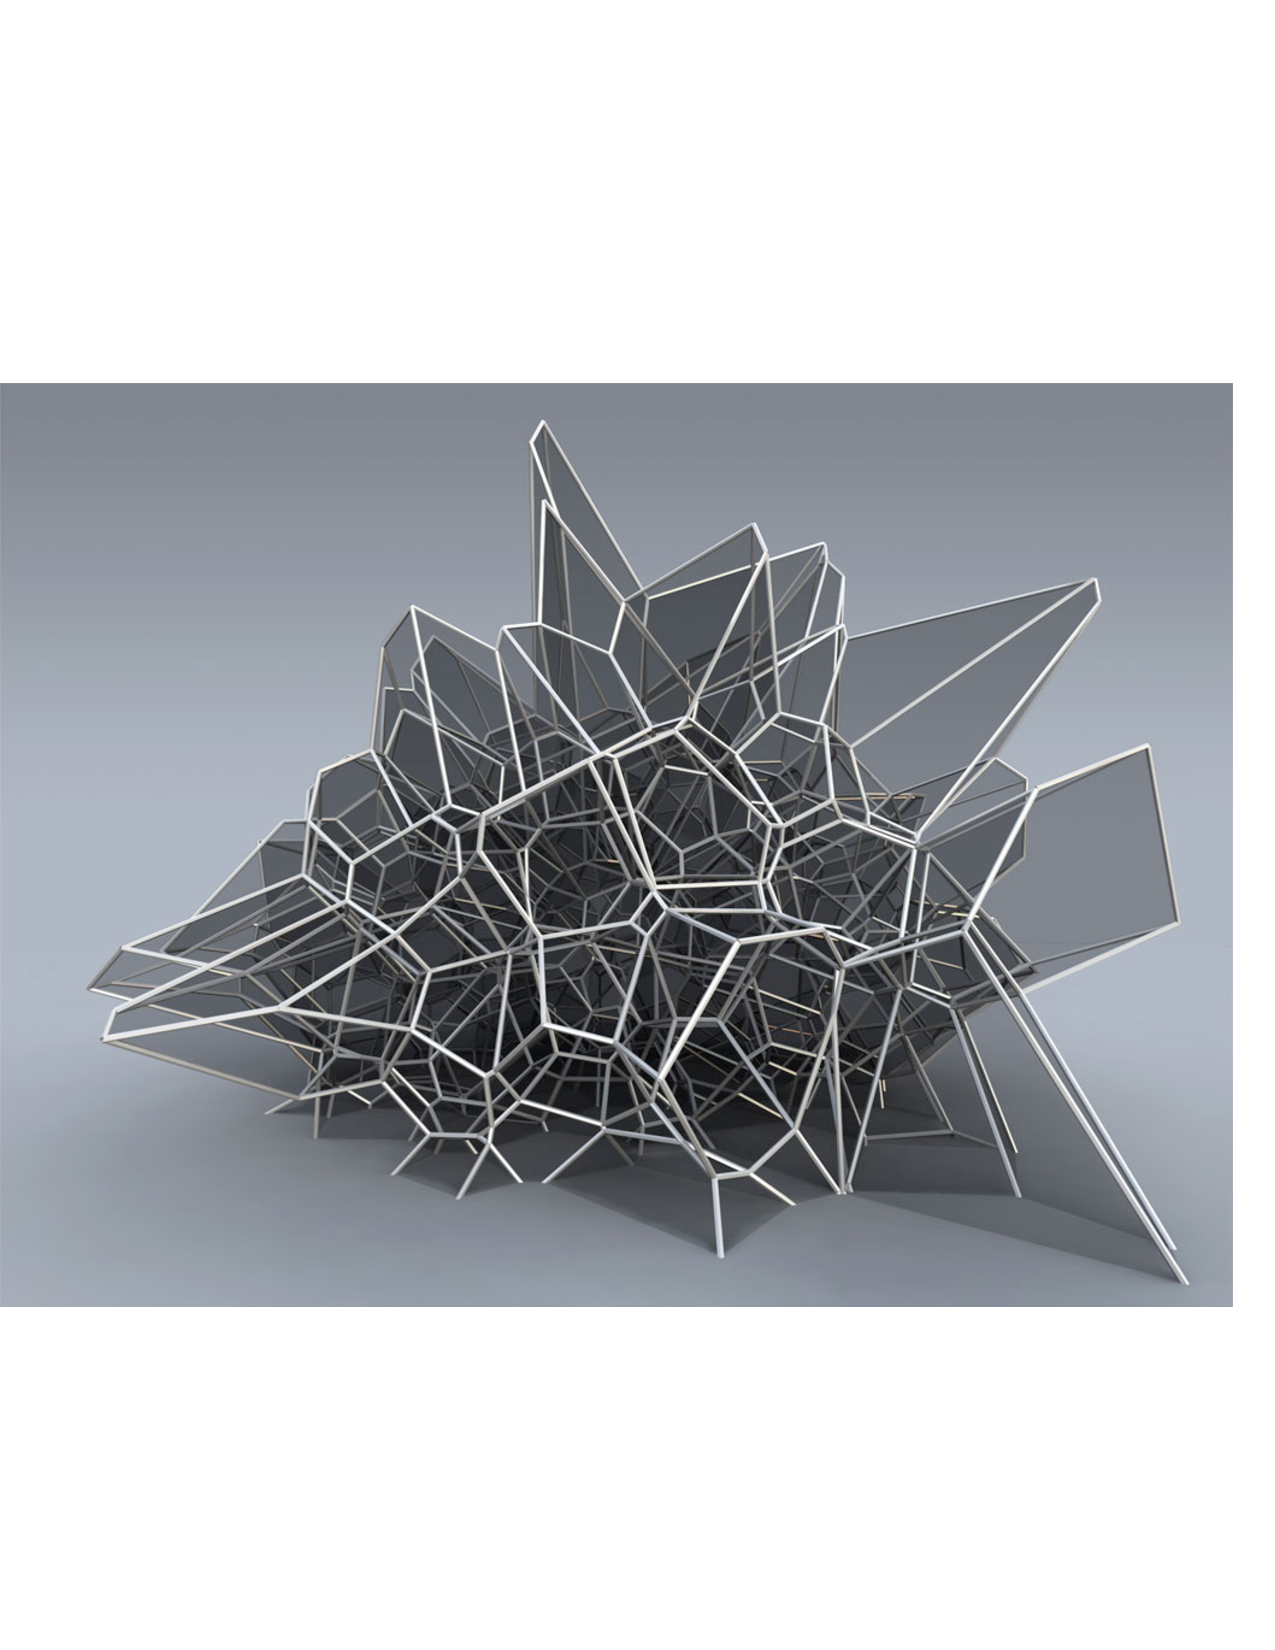
\includegraphics[scale=0.25]
  {../../../graphdod/voronoi_knauss_oesterle.pdf}
   \end{center}
  \caption{Voronoi cells.}
  \label{fig:voronoi}
\end{floatingfigure}



A packing of congruent unit radius balls 
in three-dimensional Euclidean space determines a region called the Voronoi cell 
around each ball.  
A packing is determined by and is identified  with the set $\Lambda$ of centers of the balls.  The Voronoi
cell $\Omega(\Lambda,v)$ around a ball at $v\in \Lambda$ 
consists of points of space that are closer to $v$ than
to any other $w\in\Lambda$.  The Voronoi cell is a
convex polyhedron containing $v$.

  

The Dodecahedral conjecture asserts that in any packing of congruent balls of Euclidean
space every Voronoi cell has volume at least that of a regular dodecahedron
of inradius $1$ (Figure~\ref{fig:dod}).    This bound is realized by a finite 
packing $\Lambda_{dod}$
(of twelve balls and a thirteenth  at the origin) obtained
by placing a point of $\Lambda_{dod}$ at the center of each face of a regular dodecahedron (of inradius $2$).

The
theorem can then be stated as the inequality
  $$
  \op{vol}(\Omega(\Lambda,v)) \ge \op{vol}(\Omega(\Lambda_{dod},0))
  $$
for every $v\in\Lambda$, and for every set of points $\Lambda\subset \ring{R}^3$
whose pairwise distances are at least the diameter $2$.
The case of equality occurs exactly when $\Omega(\Lambda,v)$ is
congruent to a regular dodecahedron of inradius $1$.







\subsection{history}


L. Fejes T\'oth made the conjecture in 1943 \cite{Toth1}.  
In that article, L. Fejes
T\'oth sketches a proof based on an unproved hypothesis.  This
hypothesis is a quantitative version of the kissing number problem
in three dimensions.   This unproved hypothesis
is now generally regarded as being 
nearly as difficult as the  Dodecahedral conjecture itself.  

L. Fejes T\'oth returned to the Dodecahedral conjecture in a number
of publications.  It is a prominent part of his two books \cite{Fej72},
\cite{Toth2}.  According to the strategy of \cite{Fej72}, 
the Dodecahedral conjecture forms a
step towards the solution of the sphere packing problem
(discussed below).   In \cite{Toth2}, he proved that the Dodecahedral conjecture
holds for every Voronoi cell with at most twelve faces.  
This result is reviewed in Section~\ref{sec:12sphere}.  It
is an ingredient in the proof presented here. 

%% XX This image was downloaded from the internet without permission.
% The published version needs to use a copy we own.
\begin{floatingfigure}{30mm}
  \begin{center}
  \includegraphics[scale=0.25]{../../../graphdod/dodecahedron2.pdf}
   \end{center}
  \caption{}
\label{fig:dod}
\end{floatingfigure}

A lower bound on the volume $X$ of a Voronoi cell implies
an upper bounds on the density $4\pi/(3X)$ of packings of congruent balls
in three dimensions. The Dodecahedral conjecture gives an upper
bound on density of $0.755$.  
Upper bounds on the density based on lower bounds on the volume of a Voronoi cell
literature include Rogers's upper bound 0.7797 \cite{Rogers}, and Muder's upper 
bounds 0.77836 \cite{Muder1} and 0.7731 \cite{Muder2}. 

In 1993, Hsiang published what he claimed to be proofs of the Kepler
conjecture and the Dodecahedral conjecture \cite{Hsiang}.
However, the proof did not hold up to careful analysis.  ``As of this
writing, Kepler's conjecture as well as the dodecahedral conjecture
are still unproven'' \cite[p761]{Bezdek}.  See also, \cite{Hal94}.

An alternative approach to the Dodecahedral conjecture is described
in \cite{Bezdek}.  Unfortunately, a counterexample has been found to
both parts of the third conjecture of that article.  The counterexample
is described in the preprint  \cite{arx}. 
% This
%article
%does not repeat the counterexample.


K. Bezdek conjectures that the surface area of any Voronoi cell in a packing
of unit balls is at least that of a regular dodecahedron of inradius $1$.
This strengthened version of the Dodecahedral problem is still
open \cite{Bez04}.   



\subsection{sphere packing problem}

The Kepler conjecture, also known as the sphere packing problem, 
asserts that no packing of congruent balls
in three dimensions has density greater than the density of the
face-centered cubic packing.  
S. McLaughlin carried out 
the research for the proof of the Dodecahedral conjecture 
was carried out at the University
of Michigan while S. Ferguson and T. Hales worked on the sphere packing problem.  Both
problems were solved in 1998.  

There is no strict logical connection between the two problems.
The Dodecahedral conjecture does not follow from the Kepler conjecture
and is not an intermediate step in the solution to the Kepler conjecture.
(In Fejes T\'oth's strategy, it was an intermediate step; however, that
strategy was not followed in the solution of the sphere packing problem.)
Nevertheless,
the two solutions follow a similar outline and share a significant number of 
methods.
Both are based 
on long computer calculations.  Computer
code was freely exchanged between the two projects.

This article is written in a way that it is not necessary to
read or understand the solution of the sphere packing problem before
reading this article.  However, for the benefit of the reader,
this article points  out
parallels with the sphere packing problem.  It also cites various results
from that proof.



\subsection{differences}

Although the proof of the Dodecahedral conjecture runs parallel
to the solution to the sphere packing problem, there are special
difficulties that arise in the proof of the Dodecahedral conjecture.
In no sense is it a corollary of the sphere packing problem.
In the packing problem, there turn out to be many ways to
reduce the infinite ball problem to a problem about finite clusters
of balls.  This multiplicity of choices makes it
possible to design many difficulties away.  If one reduction is
not satisfactory one can work with
another.
With the Dodecahedral problem, there is no such flexibility.
The problem about finite clusters of balls is fixed from the outset.
This gives the problem a degree of rigidity that is not present
in the sphere packing problem.


\subsection{ten years later}

Over ten years have elapsed from the completion of the research until 
publication.  A few words of explanation are in order.
The review and 
publication process for the Kepler conjecture extended from 1998
until 2006.  Because of significant sharing between the Kepler conjecture
and the Dodecahedral conjecture, a ``wait and see''
attitude developed toward the Dodecahedral conjecture.  Once the Kepler conjecture
was published, the path became clear for the publication of Dodecahedral
conjecture.  

The details of the proof in the current publication are essentially the
same as those in the preprint posted on the arXiv in 1998.  No
significant errors have emerged in the original 1998 preprint.   However,
at the request of editors,
the article has undergone three rewrites since then, an expanded version in 2002, followed by an abridged version in 2003, then a newly expanded version in 2008.  It was as if some felt a complex computer proof caused a discomfort that might be relived by a long series of
rewrites. The computer code has
also been entirely rewritten.

As an abridgment of a longer version, this article replaces 
some proofs with summaries and references.  The most complete version
is \cite{arx}.  That version is written in such a way that it is
entirely independent of the proof of the Kepler conjecture. 
This article refers the reader when necessary to relevant
passages in that proof.

A formalization project, called Flyspeck, aims to
provide a complete formalization of the proof of the Kepler conjecture \cite{fly},\cite{Fl}.  (A formalized proof is one in which every logical inference of the proof has been independently checked by computer, all the way to the primitive axioms at the foundations of mathematics.)
A parallel project, called Flyspeck Light, aims to do the same
for the proof of the Dodecahedral conjecture.  These long-term projects
will take many years to complete.  Nevertheless, significant progress
has already been made toward the formal verification of the computer
code \cite{BN}, \cite{Ob}.   The revisions in this article 
incorporate the parts of Flyspeck Light that have
already been completed.

\subsection{truncation}

The distance from the center of the regular dodecahedron to a vertex is
$t_{dod}=\sqrt{3}\tan(\pi/5)\approx 1.258$.   This parameter is used to truncate
Voronoi cells; it makes  volumes easier to estimate.  A similar truncation
takes place in the solution to the packing problem with truncation parameter
$t_0 = 1.255$.  It is a happy coincidence that these two truncation parameters 
are so close to one another.  
A great deal of duplicated effort
might have been avoided if these two parameters were equal.  However, the parameter
$t_{dod}$ cannot be replaced with anything smaller, 
and although the parameter $t_0$ could 
easily have been made larger, 
its value was already too deeply entrenched in published articles 
by the time  work started
on the Dodecahedral conjecture.  

%As a result, there are several definitions in the proof of the Dodecahedral conjecture
%and in the solution to the packing problem, identical in every respect except
%for the choice of parameter: $t_0,t_{dod}$.  This is indeed unfortunate.  However,
%there is no easy remedy. 



 As a first step towards unifying the proofs,
 many results can be stated in a form that holds for all $t\in[t_0,t_{dod}]$.
To transfer a lemma from \cite{DCG} to this article, a simple process is
involved.  The first step is generalization, replacing the constant $t_0$
with a free parameter $t\in[t_0,t_{dod}]$.  The second is specialization,
$t\mapsto t_{dod}$.  

The number $t_0$, although rational, 
can be consistently treated as an independent real transcendental 
in the solution to the sphere packing problem; that is,
none of the proofs involving $t_0$ rely on its exact numerical value.
The constant $t_0$ can always be replaced by a constant $t$
in a suitably small interval about $t_0$.  However, the only way to
know that this small interval is wide enough to contain $t_{dod}$ is to study the
details of the proof.  We have made 
a detailed study of relevant proofs in \cite{DCG} to insure that
they can be adapted to the present situation.

As a matter of terminology, a proposition for the Dodecahedral conjecture
is said to be a reparametrization of a proposition of \cite{DCG},
if it is obtained by mindlessly replacing $t_0$ with $t_{dod}$, wherever that constant appears, and if the proof goes through verbatim with this minor change.
When this occurs, 
there is nothing to further to be learned by repeating the proof.
 \cite{DCG} already contains all the needed detail.

\subsection{terminology}

Various notation and terminology is shared between the solution
of the sphere packing problem and this article.  
Vocabulary can be imported from the sphere packing problem three
different ways.  The simplest way to import a term is for the
term to have precisely the same meaning in both places.  For
example, the terms ``orientation,'' ``packing,'' have the
same meaning in both places. 

The second way to import a term is by making a reparametrization of a term that depends on the parameter $t_0$.  For example, the definition 
of standard component in this paper
is the reparametrization of standard component in \cite{DCG}.

The third way in which terms have been imported into this proof
from the proof of the Kepler conjecture has been by structural
analogy.  For example,
the term {\it tame graph} is a technical notion that arises in
the solution of the sphere packing problems.  At the analogous
point in this proof, a somewhat related collection of graphs
appears.
What to call them?  To emphasize the  analogous role they play
in the proof of the Dodecahedral conjecture, they
are called {\it tame Voronoi graphs}.  Similarly, there
is a strong analogy between Voronoi weight assignments in this
article, and admissible weight assignments in \cite{DCG}.
% structural analogy

There are a some terms in \cite{arx} that have been renamed for
greater precision.
{\it Special} has become {\it unstable}, {\it standard region}
has become {\it standard component},
{\it dihedral angle} has 
become {\it azimuth angle}, and {\it non-external} has
become {\it internal}.  {\it Planar maps} have been replaced with {\it hypermaps}.
A few terms (such as {\it distinguished}) have been slightly redefined, when doing so is harmless.


\section{Outline}

This section gives a precise statement of the main theorem
and describes the broad outline of the proof.


\subsection{formulation}\label{sec:form}

This article proves the Dodecahedral conjecture in a slightly
stronger version than that stated in the abstract. 
A  truncation of the Voronoi cell already has volume
at least as great as that of the regular dodecahedron.  This
subsection describes the truncation and states the stronger version
of the main theorem in a precise form.

Let $\Lambda$ be a packing and let $v_0\in\Lambda$.
Let $B(v_0,r)$ be an open ball
of radius $r$ centered at $v_0$. 
Let $\Lambda(v_0,r) = \Lambda\cap B(v_0,r)$.
Let $\CalS(\Lambda,v_0)$ 
be the set of all $S=\{v_0,v_1,v_2,v_3\}\subset\Lambda(v_0,2t_{dod})$
consisting of four distinct points such that $|v_i-v_j|\le 2t_{dod}$ for all $i,j$
and such that the circumradius of each triangle $\{v_i,v_j,v_k\}\subset S$ is at most
$\sqrt2$.   Write $\op{conv}(S)$ for the convex hull of $S\in\CalS(\Lambda,v_0)$. 
% and $\op{conv}^0(S)$ for its interior.
%A simple lemma (Lemma~\ref{})
%shows that distinct $S,S'\in\CalS(\Lambda,v_0)$ have disjoint
%interiors:
%   $$\op{conv}^0(S) \cap \op{conv}^0(S') \ne \emptyset 
%   \quad\Rightarrow (S = S').
%   $$


Define the following truncation $\Omega_{trunc}(\Lambda,v_0)$ 
of the Voronoi cell $\Omega(\Lambda,v_0)$:
   $$
   \{x \in \Omega(\Lambda,v_0) \mid   x\in B(v_0,t_{dod}) \quad\text{\bf  or }\quad x \in \op{conv}(S)
     \text{ for some } S\in \CalS(\Lambda,v_0) \}. 
   $$
That is, the the Voronoi cell is truncated by intersecting it with a ball of radius $t_{dod}$,
except inside regions protected by the sets $S\in\CalS(\Lambda,v_0)$.
Note that the special packing $\Lambda_{dod}$ satisfies
$\Omega_{trunc}(\Lambda_{dod},0) = \Omega(\Lambda_{dod},0)$.
The  Dodecahedral conjecture takes the following strengthened form.


\begin{theorem}\label{thm:dodec}
For every packing $\Lambda$ and every $v_0\in\Lambda$,
   $$
   \op{vol}(\Omega_{trunc}(\Lambda,v_0))\ge \op{vol}(\Omega(\Lambda_{dod},0)).
   $$
Equality holds exactly when $\Omega(\Lambda,v_0)$ is congruent to
$\Omega(\Lambda_{dod},0)$.
\end{theorem}





\subsection{proof outline}

The Lebesgue measure is translation invariant.  Thus it does no
harm to assume that the center point $v_0$ of the Voronoi cell
lies at the origin: $v_0 = 0 \in \Lambda$.  The assumption that
$v_0=0 \in\Lambda$ remains in force for the rest of this article.


The next reduction is to replace the set $\Lambda$ with $\Lambda(0,2t_{dod})$.
This is accomplished by the following lemma, which shows that the
volumes in Theorem~\ref{thm:dodec} are insensitive to points of $\Lambda$
outside $\Lambda(0,2t_{dod})$.  The proof appears in Lemma~\ref{lemma:trunc}.


\begin{lemma} Let $\Lambda$ be any packing (with $0\in \Lambda$).
Then
$$\Omega_{trunc}(\Lambda,0) = \Omega_{trunc}(\Lambda(0,2t_{dod}),0).$$
\end{lemma}

The standing assumption that $\Lambda=\Lambda(0,2t_{dod})$ remains in force
for the rest of the article.

Let $n=\#(\Lambda\setminus\{0\})$, the cardinality.
The proof of Theorem~\ref{thm:dodec}
splits into two main cases: $n\le 12$ and $n\ge 13$.
  In fact, the case $n\le 12$ was
settled by L. Fejes T\'oth in his book \cite{Toth2}.  Fejes T\'oth's proof
is sketched in Section~\ref{sec:12sphere}.

Completely different methods treat the case when $n\ge 13$.  
This part of the proof is
much more difficult than the case treated by Fejes T\'oth.
Here is a sketch of the proof of the case $n\ge 13$.   This
rough sketch will be expanded in considerably greater detail later
in the article.
Let $\Lambda$ be a packing satisfying the standing assumptions
that $0\in\Lambda$ and $\Lambda = \Lambda(0,2t_{dod})$.
The Dodecahedral conjecture seeks a minimum to the objective function 
$$
\op{vol}(\Omega_{trunc}(\Lambda,0)).
$$
This is a nonlinear optimization problem in finitely many variables.
The target value for the minimization is $\omega_{dod}=\op{vol}(\Omega(\Lambda_{dod},0))$.  When $n\ge 13$, this article proves\footnote{An examination of the proof shows the right-hand side can be improved to $\omega_{dod}+10^{-10}$.  In fact, in terms of notation to be described later in the article, the proof only
relies on the bound $\mu(\Lambda,U_F) >0$ for triangles $F$, but in fact every configuration has at least one triangle $F$ with $\mu(\Lambda,U_F) > 10^{-10}$},
   $$
   \op{vol}(\Omega_{trunc}(\Lambda,0))  > \omega_{dod}.
   $$



Some combinatorial information about each packing $\Lambda$ is encoded
as a  graph.  Let $\Lambda^* = \Lambda\setminus\{0\}$. 
The vertex set of the graph is $\Lambda^*$.
(Because of this graph,  elements of $\Lambda^*$ are generally called vertices.)
The edge set is 
  $$
  E = \{\{v,w\} \mid v,w\in\Lambda^*,\quad   |v-w| \le 2t_{dod}\}.
  $$
This is a planar graph.  
The proof reduces to the case when this graph is connected.  In fact,
when the graph is not connected, this article constructs another packing
$\Lambda'$ whose graph is connected, with the same cardinality as $\Lambda$,
and such that
$$
   \op{vol}(\Omega_{trunc}(\Lambda,0)) = \op{vol}(\Omega_{trunc}(\Lambda',0)). 
$$
Similarly, the proof reduces to the case where the graph is biconnected.
  This again involves constructing an auxiliary 
packing $\Lambda''$ of the same cardinality and whose  truncated Voronoi cell has the same volume.  Now assume that the graph of $\Lambda$ is 
biconnected.

This article supposes the existence of a counterexample $\Lambda$ to the Dodecahedral
conjecture, and makes a detailed study of the properties of its
graph.  It defines a class of graphs (called tame Voronoi) and
proves that the graph of every counterexample is tame Voronoi.

Tame Voronoi graphs can be described in purely combinatorial
terms, without reference to packings, Voronoi cells, and volumes.
All tame Voronoi graphs can be classified up to isomorphism.
This classification is one of the main steps of the proof.
There are only finitely many possibilities.  Thus, the graph
of any counterexample
to the Dodecahedral conjecture must be one of these finitely
many cases.

Each tame Voronoi graph can be encoded as a hypermap $H$.  (A hypermap can be defined
as a finite set, together with two permutations on that set.  The elements
of the given finite set are called darts.)  If $H$ is a hypermap,
let $V$ be the finite dimensional
vector space of real-valued functions on its set of darts.
The pair $(H,\Phi)$ is called a hypermap system, if $\Phi$ is a set of boolean
valued functions $\phi:V^\ell \to \{\op{true},\op{false}\}$ for
some $\ell$.
A hypermap system $(H,\Phi)$ 
is {\it feasible} if there is some $x=(x_1,\ldots,x_\ell)\in V^\ell$
such that $\phi(x)$ holds for all $\phi\in\Phi$.  Otherwise,
it is infeasible.   Appendix~\ref{ap:A} defines
a hypermap system, called the Voronoi hypermap system, 
for each case $H$ arising in the classification of
tame Voronoi graphs.

Another major step of the proof is the proof that every Voronoi hypermap
system is infeasible (Theorem~\ref{thm:graph-system}).   The proof of this theorem
is a case-by-case analysis based on the explicit enumeration of
tame Voronoi graphs, up to isomorphism.   The feasibility problem for 
each Voronoi hypermap system is converted to a system of linear programs.
The infeasibility of the Voronoi hypermap system follows from the
infeasibility of the corresponding linear program.

If there exists a counterexample to the Dodecahedral conjecture,
there is an associated Voronoi hypermap system $(H,\Phi)$.  By the preceding
result, this hypermap system is infeasible.  On the other hand, 
the counterexample can be used to construct a feasible solution to the system 
(Theorem~\ref{thm:feasible}).
This contradiction shows that a counterexample cannot exist.
In this way, the Dodecahedral conjecture is proved.







\section{Computation}

The proof of the Dodecahedral conjecture is based on a series
of computer calculations.  This section briefly describes the
computer algorithms, the code implementing those algorithms,
and issues of the reliability of the computer code.

There are three main computer programs that are used in the proof.
The first is a graph generator that generates, up to isomorphism,
 all planar graphs satisfying a list of properties.  The second is
a linear programming package.  The third is a piece of code based
on interval arithmetic that
automatically proves nonlinear inequalities over the real numbers.
This section discusses each in turn.  

This section discusses  also some
additional computer programs.  Although these computer programs,
strictly speaking, are not part of the proof, they are relevant
to understanding the structure of the proof and the reliability of
the computer implementation.   This section includes a brief discussion of
nonlinear optimization software, Tarski's decision procedure for
real-closed fields, and formal theorem proving packages.

\subsection{electronic resources}

A permanent archive has been set up for all of the external
resources related to this proof.  The URL is \cite{code}.
This archive is under version control by Google Code.  
This means that the snapshot of the archive in the
exact form it took at the time of its creation is permanently available.
It also means that any changes 
(for instance, a  bug fix) will leave
a permanent public electronic trail.
The following resources are found there.
\begin{enumerate}
\item The source code for the three different programs used in the proof (graph generation, linear programs, and interval arithmetic inequality prover)
\item A list of all tame Voronoi graphs, up to isomorphism.
\item A list of inequalities that have been established by interval arithmetic.
\end{enumerate}

\subsection{Tarski arithmetic}


The Dodecahedral conjecture, after a few preliminary reductions, 
can be expressed as a statement
in the elementary language of the real numbers.  The elementary
language of real numbers is a first order language built from
quantifiers ($\forall,\,\exists$), logical connectives ($\land,\lor,\Rightarrow,\neg$), functions symbols for ring operations ($+,\times,-$), variables $x_i$, 
and constant
symbols ($0,1$). By a fundamental
result of Tarski, the elementary theory of the real numbers
is decidable.  Thus, the
truth of the Dodecahedral 
conjecture can be decided in theory by standard
algorithms such as Collin's cylindrical algebraic decomposition \cite{Col}, or the Cohen-H\"ormander algorithm \cite{Hor}.  However,
in practice, these decision procedures are exponential time in the
number of quantifiers, and thus are far too slow to be of practical
value for this conjecture.

To formulate the Dodecahedral conjecture as a statement in the
elementary theory of the reals, consider Voronoi cells without
truncation, centered at the origin.  The
volume of the regular dodecahedron is an algebraic number $\omega_{dod}$,
hence definable in Tarski arithmetic.  Also, there are
a priori bounds $n$ on the number of faces of the Voronoi cell, and thus also
on the size of the clusters of balls that give candidates for counterexamples. (For example, by adding balls to the packing to decrease the volume, 
the  packing becomes saturated.  Assuming saturation, E. Harshbarger gives a quick calculation of $n\le58$ faces \cite{Har}. The exact value of this constant is not important as long as it is explicitly given.)
The assertion of the dodecahedral conjecture is then expressed as an enormous conjunction
of cases, with conjuncts indexed by an explicit enumeration of all possible combinatorial structures of a Voronoi cell, including a fixed triangulation of each face of the cell.  The fixed triangulation determines
a partition of the Voronoi cell into tetrahedra.  The volume of each tetrahedron is expressed by means of a Cayley-Menger determinant as a definable function of the the edge lengths of the tetrahedron.  Thus, for each combinatorial structure $X$ with $m\le 58$ faces, a Tarski statement asserts that
for all vectors $v_1,\ldots,v_m\in\ring{R}^3$, if the Voronoi cell defined by the vectors $v_i$ has combinatorial structure $X$, then the volume of the cell is at least $\omega_{dod}$.  The outer block of $3\cdot 58$ universal quantifiers -- not to mention the nested existential quantifiers -- is hopelessly beyond the practical reach of current algorithms.  The statement that the regular dodecahedron is the unique minimizer can be similarly expressed.

If the entire dodecahedral conjecture can be expressed
in Tarski arithmetic, then perhaps it is not so surprising that
many of the intermediate steps in the proof can also be so expressed.
These intermediate steps also tend to be beyond the reach of
current decision procedures.  
But here the situation is not so hopeless.  Many of these
intermediate problems involve no more than a dozen quantifiers.
One can imagine the day that these problems might fall within the
reach of decision procedures for Tarski arithmetic.

Describing various intermediate steps 
of the proof as exercises
in Tarski arithmetic is a useful point of view.  Doing so, identifies
a family of subproblems that can be expressed in a common language,
and that can often be solved by similar techniques.  
The complexity of the
problems can be measured objectively by counting the number
quantifiers.

Here are some geometrical 
objects that are definable within the Tarski arithmetic
that appear in the proof of the Dodecahedral conjecture.
The following  polynomials appear repeatedly (in the unabridged version).
\begin{definition}
$$
\begin{array}{lll}
%%\ups(x,y,z) &= -x^2 - y^2 - z^2 + 2 x y + 2 y z + 2 z x.\\ \\
 \chi(x_{ij}) &= \chi(x_{12},x_{13},x_{14},x_{34},x_{24},x_{23})\\
     &=
      x_{13} x_{23} x_{24} + x_{14} x_{23} x_{24}  + 
      x_{12} x_{23} x_{34} + x_{14} x_{23} x_{34} + x_{12} x_{24} x_{34}\\ 
      &\quad + x_{13} x_{24} x_{34} - 
      2 x_{23} x_{24} x_{34} - x_{12} x_{34}^2 
      - x_{14} x_{23}^2 - x_{13} x_{24}^2\\
   % &= x_1 x_4 x_5 + x_1 x_6 x_4 + x_2 x_6 x_5 + x_2 x_4 x_5 + x_5 x_3 x_6 \\
   %&\quad+ x_3 x_4 x_6 - 2 x_5 x_6 x_4 - x_1 x_4^2 - x_2 x_5^2 - x_3 x_6^2.\\
[0.5ex]
\Delta(x_{ij}) &= 
   -x_{12} x_{13} x_{23} - x_{12} x_{14} x_{24} - x_{13} x_{14} x_{34} 
    - x_{23} x_{24} x_{34}\\
    &\quad + x_{12} x_{34} (-x_{12} + x_{13} + x_{14} + x_{23} + x_{24} - x_{34}) \\
  &\quad + x_{13} x_{24} (x_{12} - x_{13} + x_{14} + x_{23} - x_{24} + x_{34})\\
    &\quad + x_{14} x_{23} (x_{12} + x_{13} - x_{14} - x_{23} + x_{24} + x_{34})\\
   %x_1 x_4 (- x_1+x_2+x_3- x_4+x_5+x_6)+\\&
   %         x_2 x_5 (x_1- x_2+x_3+x_4- x_5+x_6)
   %         +x_3 x_6 (x_1+x_2- x_3+x_4+x_5- x_6)
   %         - \\&x_2 x_3 x_4- x_1 x_3 x_5- x_1 x_2 x_6- x_4 x_5 x_6\\
\end{array}
    \label{def:chi}
\label{def:tar:delta}
\label{def:ups}
$$
\end{definition}

By Heron's formula, the circumradius $\eta(x,y,z)$ of a triangle with sides $x,y,z$ is elementary definable.
%$$\eta(x,y,z) = x y z/\sqrt{\ups(x^2,y^2,z^2)}.$$
Set $\eta_V(u,v,w) = \eta(|u-v|,|v-w|,|u-w|)$, for three points
$u,v,w\in\ring{R}^3$.

By Cayley-Menger determinants, the volume  of a tetrahedron with vertices $v_1,\ldots,v_4$ is elementary definable:
   $$
   \sqrt{\Delta(x_{ij})}/12,\quad x_{ij}=|v_i-v_j|^2.
   $$
In particular, $\Delta(x_{ij})\ge0$, whenever $x_{ij}$ have
the form $|v_i-v_j|^2$ for some points $v_i\in\ring{R}^3$
\cite[Lemma~8.1.4]{Part1}.

Again, if $x_{ij}=|v_i-v_j|^2$, then the orientation
of $v_1$ is said to be positive (zero, negative) in $S=\{v_1,\ldots,v_4\}$,
according to the sign of $\chi(x_{12},x_{13},x_{14},x_{34},x_{24},x_{23})$.
It is know that the sign of the orientation is positive (negative) exactly
when $v_1$ and the circumcenter of $S$ lie on the same side (opposite sides) of the
plane passing through $\{v_2,v_3,v_4\}$ \cite[Lemma~5.15]{DCG}.  This is an elementary condition. 

For $S=\{v_1,\ldots,v_r\}\subset\ring{R}^3$, let $\op{aff}_+(0,S)$
be the cone with apex $0$ generated by $S$:
  $$
  \{ t_1 v_1 + \cdots t_r v_r \mid  t_i \ge 0\}.
  $$
Write $\op{aff}_+^0(0,S)$ for the corresponding set with
strict inequality $t_i >0$.
Let $\op{conv}(S)$ be the convex hull
  $$
  \{ t_1 v_1 + \cdots + t_r v_r \mid t_i \ge 0,\ \sum_{i=1}^r t_i=1\}.
  $$
Write $\op{conv}^0(S)$ when the inequality is strict $t_i >0$.

Define the right circular cone $\op{rcone}$ by the formula
$$\op{rcone}(v,w,h) = \{x\mid (x-v)\cdot (w-v) \ge |x-v|\,|w-v| h\}.$$
%Write $\op{rcone}^0(v,w,h)$ when the inequality is strict.
For a set $S$ of fixed finite cardinality, the conditions $x\in\op{aff}_+(0,S)$,
$x\in\op{cone}(S)$, $x\in\op{rcone}(S)$ can be expressed
in the Tarski language.

In preparing this abridged version, the proofs of numerous statements
in the Tarski language (involving a small number of quantifiers) have
been omitted.  These tend to be the arguments that can most easily
be skipped without disrupting the overall flow of the proof.
The full proofs appear at \cite{arx}.



\subsection{formal proof}

A formal proof is a proof in which every logical inference has
been checked, back to the foundational axioms of mathematics. 
Except in trivial cases, a computer is used to generate a formal
proof, because of the large number of inferences involved.
Both conventional proofs and computer assisted proofs can be
formalized.  In a computer assisted proof, this amounts to a
formal verification of the correctness of the computer code.
Formal verification of computer code is a difficult task.
For that reason,  formal verification tends to be reserved
for situations where correct performance 
is critically important, such as the verification of aircraft
control systems, cryptography algorithms, 
and security protocols for the internet.
There is no other means of checking 
computer software that can assure reliability at levels that
remotely compare with the
assurance afforded by formal verification. 



There is a long term project, 
called Flyspeck Light, to give a formal verification of the
Dodecahedral conjecture.  Although this project is far from
complete, parts of this project have already
been carried out.  This means that some of the computer code
for this project now carries a proof of correctness,
according to formal mathematical standards.  One such
program is discussed in the next subsection.




\subsection{graph generation}\label{sec:gg}

The proof of the Dodecahedral conjecture is based on three separate
computer programs.  The first of these is a planar graph generator.
It generates all planar graphs, up to isomorphism, that satisfy
a given list of restrictions.  The restrictions include a bound on
the number of vertices in the graph, so that it is obvious that only finitely many graphs are possible.

The correctness of the graph generator program has been the 
subject of extensive
mathematical investigation.  Early versions of the program were
written by Hales in 1994 (in Mathematica), 1997 (in Java), and 2000 (in Java).  The same computer program is used in the Kepler conjecture
and Dodecahedral conjecture.  They differ only in their input parameters.
This computer program became the subject of  G. Bauer's
dissertation in computer science at the Technical University of Munich
\cite{Bauer}.
This 172-page dissertation translates the Java code into the
formal theorem proving system Isabelle/HOL and gives a detailed 
mathematical treatment of the graph theory underpinning the
computer code.  The dissertation analyzes every line of code.  
Building on the work of this thesis, B. Bauer
and T. Nipkow have completed the formal correctness proof of the HOL implementation
of the graph generator \cite{BN06}.  (Their published article mentions
only the Kepler conjecture, but the formal verification 
has been extended to
apply to the input parameters of the Dodecahedral conjecture as well.)
As a result of this work, the graph generation is currently the
most scrupulously checked part of the proof of the Dodecahedral
conjecture.

There are several published sources that provide details of this
algorithm, and there is no need to repeat details here.   The basic idea is to start
with a small set of planar graphs  (called `seed' graphs) with
the property that every planar graph to be classified is known to have
one of the seed graphs as a subgraph.  The seed graphs are then
extended by adding one face at a time.  Faces are added in all
possible ways so that it is clear at every step of the algorithm
that every biconnected planar graph will be generated.  At the same time,
pruning operations discard partially completed graphs when it can
be shown that the partial graph is not a subgraph of any of the
graphs to be classified.  The pruning operations prevent a
combinatorial explosion of cases.
See \cite[\S5]{alg}, \cite[\S19]{DCG}, \cite{Bauer}, \cite{BN06}.


%What it is, several implementations, bug 2000,  Mathematica, java,
%java, ML (Isabelle), formal proof of correctness.

\subsection{linear programs}

The second computer 
program that is used in the proof of the Dodecahedral
conjecture is linear programming.  There are several hundred
linear programs that appear in the proof.

Formal verification has not yet been extended to this portion
of the computer code.  However, the recent dissertation of
S. Obua takes the first steps in this direction \cite{Ob}.
That work gives a formal correctness proof of the {\it basic} linear
programs that appear in the proof of the Kepler conjecture.
In particular, he has developed all the infrastructure needed to
carry out formal correctness proofs of linear programming problems.
The formalization  completed by Obua is a larger project than the
formalization of the linear programming segment of the Dodecahedral
conjecture.
Thus, one can expect that the formalization of this piece of
computer code  will soon follow suit.

In the 1998 proof, computer code written in C  generated 
the linear programs, which were then fed to the 
commercial linear programming
package CPLEX.  In preparation for a formal proof, the computer
code has been rewritten in the programming language ML, with
an external interface to the solver GLPK.

It is not necessary to trust the algorithms of the
linear programming packages (such as CPLEX and GLPK) that solve
the linear programs.  These packages produce dual certificates that
can be used to give independent verification of the solutions
of the linear programming problems.

In the proof of the Dodecahedral conjecture,   the
following situation arises.  The objective is 
to prove that the maximum of a
linear function 
$x\mapsto c x$ is less than a given constant $M$, when subject
to a system of linear constraints $A x \le b$.  (Here $x$, $c$, $b$
are vectors with real entries and $A$ is a matrix with real
entries.  The products are given by matrix multiplication of compatibly sized matrices and vectors. 
A vector inequality $u\le v$
means that $u_i \le v_i$ for each coordinate $i$.) 
Explicit lower and upper bounds on the variables
are given: $\ell \le x \le u$.
Expressed equivalently, the objective is to show that the linear 
system of inequalities
  $$
  A x \le b,\quad \ell \le x\le u,\quad c x \ge M
  $$
has no solutions in $x$.
The external linear programming package produces a dual certificate
in the form of a vector $y$, which that package claims to have
the properties 
  \begin{equation}
  y A = c,\quad y\ge 0,\quad y b < M.
  \end{equation}
If $y$ indeed has these properties, then for any $x$ satisfying
$A x \le b$, it follows that
   \begin{equation}\label{eqn:cxM}
   c x = y A x \le y b < M
   \end{equation}
as desired.

Because of inexact arithmetic used by the external packages, 
these identities will only be
approximately correct.   The imprecision in the dual
certificate can be readily eliminated as follows. If $u$ is
any vector, let $u^+$ be the vector obtained by replacing the
negative entries of $u$ with $0$, and let $u^-$ be the vector
obtained by replacing the positive entries of $u$ with $0$.
By replacing the vector $y$ with $y^+$, the vector $y$ satisfies
$0\le y$.  In the following lemma, $\epsilon_1$ and $\epsilon_2$ are
small error terms that result from machine approximation.
By including them in the bounds on $c x$, a rigorous bound
can be recovered.


\begin{lemma}  Suppose that the real-valued vectors and matrices
$A,A_1,A_2$, $c,c_1,c_2$, $x,b,\ell,u$, $y$ satisfy the following
relations
  $$
  A x\le b, \quad A_1 \le A \le A_2,
  \quad c_1 \le c \le c_2,\quad \ell\le x\le u,\quad
  0\le y.
  $$
Define residuals
  $$
   \epsilon_1 = c_1 - y A_2,\quad \epsilon_2 = c_2  - y A_1.
  $$
If
$$
y b + \epsilon_2^+ u^+ + \epsilon_1^+ u^- + \epsilon_2^- l^+ + \epsilon_1^- l^- < M,
$$
then $c x < M$.
\end{lemma}

\begin{proof}  S. Obua has given a formal proof of this lemma in
the Isabelle/HOL system \cite[3.7.2]{Ob}.  In fact, the proof is
nothing but a slight
embellishment of Inequality~\ref{eqn:cxM}.
\end{proof}

The numerical data $A_1,A_2,c_1,c_2,\ell,u,y,b$ are all explicitly given,
so that explicit bounds are obtained by this
method.  It is not necessary to trust the package
that produces the certificate $y$, because
all of the assumptions of the lemma can be checked directly with
simple matrix multiplications.  The reliability of these matrix
multiplications can be guaranteed by using interval arithmetic.\FIXX{Has this been checked with interval arithmetic?}


\subsection{interval arithmetic}

The third major computer program that is used in the proof of
the Dodecahedral conjecture is an nonlinear-inequality prover
over the real numbers based on interval arithmetic.  
This subsection describes the
methods involved and the computer implementation.

A finite number of nonlinear functions $f_1,\ldots,f_r$ are given.
It is assumed that all functions have the same domain
   $$R= [a_1,b_1] \times [a_2,b_2] \times [a_m,b_m],$$
given as a product of intervals in $\ring{R}^m$, for some $m$.
The computer program verifies that
  \begin{equation}\label{eqn:fpos}
  (f_1(x) >0) \lor (f_2(x) >0) \lor \cdots \lor (f_r(x) >0),
  \end{equation}
for every point $x\in R$.
The approach is similar to the approach described in
R. B. Kearfott \cite{Kea96}, based on interval arithmetic.
Our methods are similar to algorithms in widespread use for
rigorous global optimization.  Closely related algorithms
are also described in \cite{Zu}.

The method is based on an iteratively refined 
partition of the domain  $R$
into a finite number of smaller and smaller rectangles that cover $R$.

Start with $X=\{R\}$,  then repeat the following procedure.
Pick $T\in X$; replace $X$ with $X\setminus\{T\}$; and
calculate a lower bound $f_j(x) > a_j(T)$, 
for all $x\in T$.  If $a_j(T)\ge 0$ for some $j$, then
the desired bound holds.  Repeat for the next rectangle in $X$.
Otherwise, choose finitely many rectangles, $T_1,\ldots,T_k$ that cover $T$;
replace $X$ with $X\cup\{T_1,\ldots,T_k\}$, then repeat.
The procedure terminates when $X=\emptyset$.  (If the procedure
is applied to a false disjunction (\ref{eqn:fpos}), there is no
termination.)

% Grothendieck topologies again!
%Here is a somewhat simplified description of the algorithm.
%At iteration $p$,   $R$ is covered by smaller rectangles
%$R^p_1,\ldots,R^p_{k_p}$, and lower bounds are calculated on each $R^p_{i}$
%   $$
%   f_j(x) > a_{p,i,j},\quad \text{ for } j=1,\ldots,r;\quad i=1,\ldots,k_p.
%   $$
%If $a_{p,i,j}\ge 0$ for some $j\le r$, then the condition~\ref{eqn:fpos}
%holds for $x\in R^p_i$.  
%If for every $i$, there exists a $j$ such that $a_{p,i,j}\ge 0$,
%then condition~\ref{eqn:fpos} holds for $x\in R$, and the algorithm
%terminates.

%If not, pick $i' \le k_p$ for which no such $j$ exists and
%pass to the next iterate $p+1$ of the algorithm.  Cover $R^p_{i'}$
%with finitely many rectangles $S^{p+1}_1,\ldots$, and let
%  $$
%  R^{p+1}_1,\ldots,R^{p+1}_{k_{p+1}}
%  $$
%be the collection consisting of $S^{p+1}_1,\ldots$ and $R^p_1,\ldots$
%(omitting $R^p_{i'}$).  New lower bounds $a_{p+1,i,j}$  are computed
%for $f_j$ on each new rectangle, and continue as before.

When subdividing rectangles to obtain smaller covers, one does
it in such a way the the width of the rectangle tends to zero
as iteration continues.
In this way,  the lower approximations 
$a_j(T)$ to $f_j$ can be arranged to converge to the true minimum of $f_j$ on the
rectangle.

The lower bounds $a_j(T)$ to a function $f_j$ on a rectangle $T$
are obtained by methods of interval arithmetic.  The function
$f=f_j$ is generally $C^2$ on its domain.\footnote{The functions
 encountered in practice are usually $C^2$, but not always so.  When functions are not
$C^2$,  Taylor approximations are avoided.}  
The function $f$ can be expanded in a Taylor polynomial approximation with
explicit error bounds.  Derivatives are calculated by automatic
differentiation.  The error bounds are based on the Lagrange form of
the error term in the Taylor approximation.  Interval arithmetic is used to produce rigorous bounds on the error terms.

%We take comfort in the fact that we have
%been able to give rigorous proofs of difficult inequalities,
%especially when confronted with the fact that 
%nonlinear optimization is NP hard.  Considerable work has gone
%into the implementation of these algorithms.

There have been several separate implementations of the interval
arithmetic package.  
The source code for all of these packages
is publicly available. (The code that is used for the proof of 
the Kepler conjecture is the same as the code that is used for
the proof of the Dodecahedral conjecture.  Only the statements
of the inequalities to be proved differ.) 
The first version, written in C++, 
was developed by T. Hales
over the period 1994-1998.  
A second version, written in C, was developed by S. Ferguson 
1995-1997.  A third version, written in ML, was developed by S. McLaughlin 2006-2008.  A interval arithmetic package has also been developed
by R. Zumkeller for the theorem proving system COQ, although it has not  been used to give a formal verification of any of the inequalities that arise in the proof of the Dodecahedral conjecture \cite{Zu}.
These implementations are all independent of one another. (Algorithms
were shared among us, but the code was independently implemented.) 
By comparing the proofs of different inequalities in different 
systems, we have developed 
a high degree of confidence that the implementations
of the algorithms are essentially correct.  Of course, it would
be desirable to have a formal correctness proof, but this part
of the Flyspeck Light project has not been completed.  (The ML
implementation and Zumkeller's research are partial steps
in this direction.)

The list of nonlinear inequalities that are used in the
proof of the Dodecahedral conjecture appears at \cite{code}.
The domains of the functions are subsets of $\ring{R}^m$, for
$m\le 7$.  The complexity of the verification increases
rapidly with $m$.  This proof implements  some of the tricks introduced
in \cite{DCG} to reduce the dimension of the domain wherever
possible.  Dimension reduction is based on established
monotonicity properties of the functions.  (For example, the
volume of a Voronoi cell does not increase when it is intersected
with a half-space.)  Whenever the functions $f_j$ are twice continuously
differentiable,  a first order Taylor polynomial with
explicit error bounds on the second derivatives is used. 
The functions $f_j$ represent elementary geometric quantities such
as linear combinations of angles, dihedral angles, solid angles,
and volumes.  Explicit formulas for these functions are known
involving rational functions, the square root, and $\arctan$ functions.
The typical form of a function $f_j$ is a linear combination of terms
of the form
    $$
    \arctan(a/\sqrt{b}),
    $$
where $a,b$ are explicit polynomials on $\ring{R}^m$.
In the 
formula (\ref{eqn:fpos}), the number of disjuncts is usually one
$r=1$, but in some cases there are two disjuncts.

The computer calculations use interval arithmetic to
control for floating-point round-off errors.  Every real number $x$
is represented on the computer as an interval $[a,b]$ containing $x$, where $a$ and $b$ are
exactly representable floating point numbers \cite{Interval}, \cite{Numerics}.
The calculations conform to IEEE-754 standards \cite{Float}.
Approximations to inverse trigonometric functions are based on 
published approximations \cite{Approx}.



\subsection{nonlinear optimization}

Previous subsections describe the three main pieces of computer
code used in the proof of the Dodecahedral conjecture: graph 
generation, linear programming, and interval-arithmetic inequality
proving.  This subsection describes one additional software
package indirectly involved in the proof: nonlinear-optimization.  
This package was used only in a heuristic way
and does form part of the proof tree.

The disjunction of inequalities in formula (\ref{eqn:fpos}) can
be represented as a constrained minimization problem: show that
the global minimum of $f_1$ on the domain
$$
\{x\in[a_1,b_1]\times\cdots\times[a_m,b_m] \mid  f_2(x)\le 0,\ldots,
  f_r(x)\le 0 \}
$$
is positive. Nonlinear optimization packages have been
used to test the validity of the constrained minimization
problems in the collection.

The nonlinear optimization library {\it cfsqp} has been used to
test all the inequalities in the collection \cite{cfsqp}.  
The algorithm
is based on sequential quadratic programming, which
searches for a local minimum of an objective function
according to a quadratic model of the objective
function.  The code generates a large random set $X$ of points in the
domain and runs the algorithm for each initial point $x\in X$ to
find a local minimum to the objective function $f_1$.  If $X$
is sufficiently large and sufficiently random, it can
be expected that one
of the local minima produced to be a numerical approximation
of the  global minimum.

In practice, this approach works remarkably well on this
collection of problems, largely because the functions $f_j$
tend to be rather bland from the point of view of nonlinear
optimization.  (Typically, the second derivatives of $f_j$
are small; the level surfaces of $f_j$ are approximately planar;
there are no local minima in the interior of the domain;
the global minimum occurs at a corner of the domain; and
every run of the algorithm produces the same local minimum.)
Thus, the method can usually determine the true global minimum with
high probability.


If this nonlinear optimization is not part of the proof tree,
what purpose does it serve? First of all, although we have
tried to be careful to avoid any errors in the computer code,
an independent check of the results is certainly welcome.
It makes the proof more robust against possible errors.  
In fact,
this independent check has helped us to spot and correct 
 data entry errors.  Secondly, the package was used to discover
inequalities that were likely to be true, and to discard quickly
inequalities that were false.  The plausibly true inequalities
then became candidates for  rigorous nonlinear optimization
with interval arithmetic.

More recently, 
S. McLaughlin has produced Objective CAML bindings for the
cfsqp library \cite{McLp}.  The nonlinear inequalities in this
collection have also been retested with a second package
Knitro.  This package implements a variety of algorithms
(barrier techniques, conjugate gradient methods, an active set algorithm).


\subsection{summary}

This section has described various computer programs 
and algorithms that
have been used in the proof of the Dodecahedral conjecture.
The rest of the article assumes that the types of
computations described in this section can be reliably performed
by computer.

Recall briefly how the three main computer programs
enter into the proof.  A planar graph is associated with
each potential counterexample of the Dodecahedral conjecture.
The properties of this graph is studied, and it is shown to
be a tame Voronoi graph.  Using the graph generator program,
all such graphs are classified up to isomorphism.  This
reduces the proof to a finite enumeration of cases. Linear programs
are then used to show that each case in this enumeration is 
infeasible.  The nonlinear inequalities appear in several different
parts of the proof.
They are used, for example to establish that the graph associated
with a counterexample is a tame Voronoi graph.  Nonlinear
inequalities are also used to justify the list of inequalities
used in the linear programs. (The linear programming inequalities
come as linear relaxations of nonlinear inequalities.)



\section{Fejes T\'oth's Reduction}\label{sec:12sphere}

L. Fejes T\'oth proved  the Dodecahedral conjecture 
under the extra hypothesis that $\Lambda(v_0,2t_{dod})\setminus\{v_0\}$
has at most $12$  elements.  The proof occupies about
eight pages of the book {\it Regular Figures}.  See the main
theorem of
Section~33 and the main theorem of Section~41 (including
the note on page 265) in \cite{Toth2}.  Fejes T\'oth's
bound is a general bound about the volume of truncated polyhedra.
The polyhedra do not have to be Voronoi cells in a sphere packing.
Here is a sketch of his proof.

\begin{theorem}  Let $P$ be any polyhedron with at most $12$ faces
that contains a unit sphere $S^2$.  Let $B$ be the ball of
radius $t_{dod}$ concentric with $S^2$.  The volume of the intersection
of $P$ with $B$ is
at least that of a regular
dodecahedron $D$ with inradius $1$.
Equality holds exactly $P$ is congruent to $D$.
\end{theorem}

\begin{proof} (Sketch)  By translation, the proof reduces to
the case that the origin is the center of $S^2$.
If $k<12$, there is a polyhedron with smaller volume and $k+1$ faces,
obtained by clipping a corner of the polyhedron with a new face.
Thus, assume $k=12$.  
View the case in which some vertices of the polyhedron
have degree greater than $3$ as degenerate cases of polyhedra 
where all degrees are three, where some of the vertices have
coalesced.   With these conventions, 
there are $12$ faces, $30$ edges,
and $20$ vertices.

Let 
  $$g(x) = \begin{cases}
          \frac13 \sec^2 (x), & x \le \theta_0\\
          \frac13 \sec^2 (\theta_0), & x \ge \theta_0,
          \end{cases}
   $$
where $\theta_0$ is defined by $\sec(\theta_0) = t_{dod}$.
For each face $F_i$ of the polyhedron $i=1,\ldots, 12$, 
let $w_i$ be the point 
on the unit sphere $S^2$ at the origin closest to the plane through $F_i$.
Let $S_i$ be the radial projection of $F_i$ to a spherical polygon
on $S^2$.   The volume $\omega$ of the $t_{dod}$-truncated polyhedron satisfies
    \begin{equation}\label{eqn:V}
    \omega \ge \sum_{i=1}^{12} \int_{S_i} g(\theta(w_i,x))\,dx
    \end{equation}
where $dx$ is the usual measure on $S^2$,
and $\theta(w_i,x)$ is the geodesic length of the arc on $S^2$ joining
$w_i$ to $x$. The integral on the
right is exactly the volume of the truncated polyhedron obtained
by projecting each polygon $S_j$ back out to a plane parallel to $F_i$
through $w_i$.

By the estimate of Sec.~33 of the book, 
the integral on the right is at least
   $$
   120 \int_{T} g(\theta(w,x))\, dx,
   $$
where $T$ is a spherical triangle with angles $\pi/2$,
$\pi/5$, $\pi/3$.  Here $w$ is the vertex of the triangle $T$
that has angle $\pi/5$.  (This estimate 
holds in fact for any non-decreasing function $g$.)

This integral is precisely the volume of a regular
dodecahedron of inradius $1$.  Indeed, when the polyhedron
is a regular dodecahedron,  the maximum of $\theta(w,x)$ over the pentagon 
$S_i$ is exactly $\theta_0$.  (This fact is equivalent to the definition of $t_{dod}$ as the circumradius of the regular
dodecahedron, so that no truncation occurs.)
So $g(|w-x|) = (\sec^2\theta(w,x))/3$.  The inequality (\ref{eqn:V})
is an equality.  Also, each regular pentagon $S_j$ can be triangulated
into $10$ triangles with angles $\pi/5$, $\pi/2$, $\pi/3$.  The
$12$ faces then give $120$ triangles $T$.  The result follows.

L. Fejes T\'oth also considers the case of equality and finds that
the only minimizing polyhedron is the regular dodecahedron.
\end{proof}



%XXP Proof read to here.


\section{Geometry of Voronoi Cells}

This section describes the basic geometry of the
 Voronoi cell and
its truncation.  

\subsection{basic truncation}\label{sec:in-ex}

Let $\Lambda = \Lambda(0,2t_{dod})$ be a finite
packing containing $0$, and let $\Omega(\Lambda,0)$ be the Voronoi cell.
Let $B(x,r)$ be the open ball of
radius $r$ centered at $x\in\ring{R}^3$.
Let $\Omega_0(\Lambda,0) = \Omega(\Lambda,0)\cap B(0,t_{dod})$.
Also, $\Omega_{trunc}(\Lambda,0)$ 
has been defined in Section~\ref{sec:form}.

%% Repeat. 
Recall $\Lambda^* = \Lambda\setminus\{0\}$.  There is a graph $G(\Lambda)$
with vertex set $\Lambda^*$, whose edges are formed by pairs
$\{v,w\}$ such that $0<|v-w|\le 2t_{dod}$.  Figure~\ref{fig:icos}
shows the regular icosahedron, which is the graph $G(\Lambda_{dod})$.


%% XX This image was downloaded from the internet without permission.
% The published version needs to use a copy we own.
\begin{floatingfigure}{30mm}
  \begin{center}
  \includegraphics[scale=0.18]{../../../graphdod/icosahedron2.pdf}
   \end{center}
  \caption{}
\label{fig:icos}
\end{floatingfigure}

The geometry of $\Omega_0(\Lambda,0)$ will be discussed first,
then adapted to $\Omega_{trunc}(\Lambda,0)$.  The truncated cell
$\Omega_0(\Lambda,0)$ is obtained from the ball $B(0,t_{dod})$ by
removing a spherical cap
   $$
   C(v,t_{dod}) = \{x \in B(0,t_{dod}) \mid  |x - v| \le |x| \}
   $$
for each $v\in\Lambda^*$.
Each spherical cap is bounded by a sphere of radius $t_{dod}$ and
a planar disk formed by the intersection of the bisector of 
$\{0,v\}$ with the ball $B(0,t_{dod})$.
We need the following functions, where $\lambda=(\lambda_v,\lambda_s)$:
\begin{equation}
\begin{array}{lll}
\phi(h,t,\lambda) &= \lambda_v t h (t+h)/6 + \lambda_s\\
A(h,t,\lambda) &= (1-h/t)(\phi(h,t,\lambda)-\phi(t,t,\lambda))\\
\end{array}
\end{equation}
When $\Lambda^* = \{v\}$ has a single point, the truncated Voronoi
cell is a ball of radius $t_{dod}$
with a single cap $C(v,t_{dod})$ removed.  Its volume depends
only on $|v|=2h$ (and $t_{dod}$).  
The cone at the origin generated by the points of $C(v,t_{dod})$ is
$\op{rcone}(v,h/t_{dod})$.  An elementary calculation gives the volume and
solid angle formulas.
\begin{equation}  
\begin{array}{lll}
\op{vol}(C(v,t_{dod})) &= \phi(h,t_{dod},(1,0)) \\
\op{sol}(\op{rcone}(v,h/t_{dod})) &= \phi(h,t_{dod},(0,1)).\\
\end{array}
\end{equation}



When $\Lambda^*=\{v,w\}$ contains two points, the two spherical
caps meet if and only if $\eta_V(0,v,w) < t_{dod}$.  (Recall that
$\eta_V$ denotes the circumradius.)   The volume formula for
$\Omega_0(\Lambda,0)$ as a function of $v,w$ is continuous
across the level curve $\eta_v(0,v,w)=t_{dod}$, but not analytic.
When $\eta_v(0,v,w) > t_{dod}$ the caps are disjoint and the
volume is independent of $|v-w|$, depending only on $|v|$ and $|w|$.
That is, the volume does not depend on the location of the caps,
provided they are disjoint.

When $\eta_V(0,v,w) < t_{dod}$, the volume depends on
$|v|,|w|,|v-w|$.  Note that $\eta_V(0,v,w) < t_{dod}$ implies
$|v-w|\le 2t_{dod}$, so that the graph $G(\Lambda^*)$ contains
the edge $\{v,w\}$.
By inclusion-exclusion, the volume of $\Omega_0(\Lambda,0)$ is
   \begin{equation}\label{eqn:in-ex}
   \op{vol}(B(0,t_{dod})) - \op{vol}(C(v,t_{dod})) - \op{vol}(C(w,t_{dod})) +
 \op{vol}(C(v,t_{dod}) \cap C(w,t_{dod})).
   \end{equation}
The set $C(v,t_{dod})\cap C(w,t_{dod})$ can be partitioned
into four regions (called quoins)
Let $P_1$ be the plane through $0,v,w$.  Let $P_2$ be the
plane orthogonal to $P_1$ that passes through $0$ and the circumcenter
of the triangle $\{0,v,w\}$.  Then $\ring{R}^3\setminus (P_1\cup P_2)$ 
contains four connected components, partitioning $C(v,t_{dod})\cap C(w,t_{dod})$
into four quoins.  
Let $a=|v|/2$, $b=\eta_V(0,v,w)$, $c=t_{dod}$.  Let $q(a,b,c)$ be the
volume of the quoin given by the intersection
  $$C(v,t_{dod})\cap C(w,t_{dod}) \cap H_1 \cap H_2,
  $$
where $H_1$ is a half-space bounded by $P_1$ and $H_2$ is
the half-space bounded by $P_2$ containing $w$.
The volume of a quoin is computed in \cite[7.3]{DCG}.
If $a\le b\le c$, then 
\begin{equation}
\begin{array}{lll}
6 \op{quo}(a,b,c) &= (a+2c) (c-a)^2 \arctan(e) + a(b^2-a^2) e \\
&\quad - 4c^3 \arctan(e(b-a)/(b+c)),\text{ where}\\ [0.5ex]
e^2 (b^2-a^2)&= (c^2 - b^2), \quad \text{ and } e\ge 0.
\end{array}
\end{equation}
Otherwise, $\op{quo}(a,b,c) = 0$.  By (\ref{eqn:in-ex}), this gives
the volume of $\Omega_0(\Lambda,0)$ when $\Lambda^*=\{v,w\}$.





When $\Lambda^*=\{v_1,v_2,v_3\}$ contains three points, the three spherical
caps meet if and only if the circumradius of the simplex
$\{0,v_1,v_2,v_3\}$ is less than $t_{dod}$.  When this happens, each
edge $|v_i-v_j|\le 2t_{dod}$, so that the graph $G(\Lambda)$ is a
triangle.  Also, the circumradius of each face is at most
$t_{dod} < \sqrt2$.  Thus, 
  $$\{0,v_1,v_2,v_3\}\in\CalS(\Lambda,0).$$
These are the sets singled out for special truncation in $\Omega_{trunc}$.
%se return to this in a moment.

If the three spherical caps do not meet or meet in at most pairs,
then the volume, by inclusion-exclusion is given by a formula
similar to (\ref{eqn:in-ex}).  In particular, the volume
is given in terms of quoins, and so forth.

The case when the graph $G(\Lambda)$ is connected, but not a triangle
has particular interest.  Suppose that there is no edge between
$v_1$ and $v_3$. In this case, the volume of $\Omega_0$ depends on
$|v_i|$, $|v_1-v_2|$ and $|v_2-v_3|$, but not on $|v_1-v_3|$.
Thus, the point $v_3$ can be moved, subject to the constraints
fixing $|v_3|$ and $|v_2-v_3|$ without changing the volume.
In particular, $v_3$ can be moved until $|v_3-v_1|=2t_{dod}$.  This
results in the following simple lemma.  

\begin{lemma}\label{lemma:3tri}  
Suppose $G(\Lambda)$ contains three vertices,
is connected, but not a triangle.  Then there is another packing
$\Lambda_1$ whose graph $G(\Lambda_1)$ is a triangle and such
that
  $$
  \op{vol}(\Omega_0(\Lambda,0)) = \op{vol}(\Omega_0(\Lambda_1,0)).
  $$
\end{lemma}

The same lemma holds
for $\Omega_{trunc}$ because in the situation at hand $\Omega_0=\Omega_{trunc}$.
Lemma~\ref{lemma:4fold} shows it is not possible for four or more
spherical caps to meet.

\subsection{planarity}

\begin{definition}[spherical]
For each edge $e=\{v,w\}$ of a graph $G(\Lambda)$,
let $A_e$ be the arc on the unit sphere at the origin formed
by the intersection of the sphere with $\op{aff}^0_+(0,\{v,w\})$.
Any graph $G'$ on the edge set $\Lambda^*$, is called
{\it spherical} if the sets $A_e$ do not meet one
another, as $e$ runs over the edges of $G'$.  
\end{definition}

A spherical graph is clearly a planar.

\begin{lemma}\label{lemma:planar}  
$G(\Lambda)$ is a spherical graph.
\end{lemma}

\begin{proof}  It suffices to show that the sets
$\op{aff}^0_+(0,\{v,w\})$ do not meet one another, as $e=\{v,w\}$
runs over edges.  This is a statement in Tarski arithmetic.
A detailed proof appears in \cite[Lemma~3.2]{arx}.  
It is the reparametrization
of the published theorem \cite[Lemma~3.10]{Part1}.
\end{proof}


\subsection{triangles}

This subsection describes the geometry associated with
triangles in the graph $G(\Lambda)$.  For each triangle,
there is a set $\{0,v_1,v_2,v_3\}$ such that
\begin{equation}\label{eqn:qrtet}
  |v_i| \le 2t_{dod},\quad |v_i-v_j | \le 2 t_{dod},\quad i,j\le 3.
\end{equation}

\begin{lemma} Let $S=\{0,v_1,v_2,v_3\}$ be a set of four points
that satisfies (\ref{eqn:qrtet}).  Then
there does not exist $w\in\op{conv}(S)$
(the convex hull of $S$) that satisfies $|w-u|\ge 2$ for all
$u\in S$.
\end{lemma}

\begin{proof}  This is a statement in Tarski arithmetic 
that can be expressed with $12$ quantifiers ($3$ coordinates
for each of $v_1,v_2,v_3,w$).  The proof is
the reparametrization of \cite[Lemma~4.15]{DCG}.
It is written out in full in \cite[Lemma~3.3]{arx}.
\end{proof}

\begin{lemma}\label{lemma:enclosed} 
Let $S=\{0,v_1,v_2,v_3\}$ be a set of four points
that satisfies (\ref{eqn:qrtet}).  Then
there does not exist $w\in\op{aff}_+(0,\{v_1,v_2,v_3\})$
(the cone with apex $0$ 
generated by positive linear combinations of $v_i$) 
that satisfies $|w-u|\ge 2$ for 
$u\in S$ and $|w|\le 2t_{dod}$.
\end{lemma}

\begin{proof} This is a statement in Tarski arithmetic.
The case when $w\in\op{conv}(S)$ is covered by the previous lemma.
The remaining case is a reparametrization of
\cite[Lemma~4.19]{DCG}.  See also,  \cite[Cor~3.7]{arx}.
\end{proof}

\begin{lemma}\label{lemma:4fold}  
Let $0,v_1,v_2,v_3,v_4\in\Lambda$, with
$v_i$ distinct.  The intersection $\cap_{i=1}^4 C(v_i,t_{dod})$
of spherical caps is empty.
\end{lemma}

\begin{proof}  A nonempty intersection implies that each
edge $\{v_i,v_j\}$ in  $G(\Lambda)$, forming a complete graph
on four vertices.  The graph is planar by Lemma~\ref{lemma:planar}.
Its planar representation is a triangle with one vertex inside,
connected to all three vertices of the triangle.
Geometrically, this corresponds to a point $v_4\in\op{aff}_+(0,\{v_1,v_2,v_3\})$, which is impossible by the previous lemma.
\end{proof}

\begin{lemma}  Let $\{v_1,v_2,v_3\}$ and $\{v_1',v_2',v_3'\}$
be two distinct triangles in $G(\Lambda)$.  Then
$\op{aff}_+^0(0,\{v_1,v_2,v_3\})$ is disjoint from
$\op{aff}_+^0(0,\{v_1',v_2',v_3'\})$.  In particular,
$\op{conv}(\{0,v_1,v_2,v_3\})$ is disjoint from
$\op{conv}(\{0,v_1',v_2',v_3'\})$.
\end{lemma}

\begin{proof} Since the graph is planar, if the two cones
intersect, then one triangle must be contained in the other
triangle.  That is, one cone is contained in the other.  This
leads to a vertex $w$ of one triangle in the other
cone.  This is prohibited
by Lemma~\ref{lemma:enclosed}.
\end{proof}

As mentioned earlier, a three-fold intersection of spherical
caps produces a triangle in the graph $G(\Lambda)$ and a 
set 
$$\{0,v_1,v_2,v_3\}\in \CalS(\Lambda,0).$$
The next two lemmas investigate the geometry of such $\{0,v_1,v_2,v_3\}$.

\begin{lemma}\label{lemma:Q}
If $S=\{0,v_1,v_2,v_3\}$ is a set of four points such that each
face has circumradius at most $\sqrt2$ and such that
$|u-v|\le 2t_{dod}$ for $u,v\in S$, then
the circumcenter of $S$ lies in $\op{conv}(S)$.  Also, if $x
\in \op{conv}(S)$ and $w$ has distance at least $2$ from each
point of $S$, then $x$ is at least as close to some point of $S$ than to
$w$.
\end{lemma}

\begin{proof} This is a statement in Tarski arithmetic.
The statement about the circumcenter is \cite[Lemma~5.18]{DCG}.
(No reparametrization is needed.)
If $x$  comes closer to  to $w$  than to each point of $S$, then
the Voronoi cell $\Omega(S\cup\{w\},w)$ meets $\op{conv}(S)$.
Again by \cite[Lemma~5.18]{DCG}, this implies that the circumradius
of some face of $S$ is greater than $\sqrt2$, which is contrary
to hypothesis. An alternative proof 
of both parts of the lemma
is contained in \cite[Lemma~3.5,3.6]{arx}.
\end{proof}

The following lemma justifies limiting packings to those
satisfying $\Lambda=\Lambda(0,2t_{dod})$.  Extending the packing
$\Lambda$ beyond radius $2t_{dod}$ cannot decrease the volume of the
truncated Voronoi cell.

\begin{lemma}\label{lemma:trunc}  
Let $\Lambda=\Lambda(0,2t_{dod})$.  Let $\Lambda\subset\Lambda'$,
where $\Lambda'(0,2t_{dod}) = \Lambda(0,2t_{dod})$.  Then
$$\Omega_{trunc}(\Lambda',0) = \Omega_{trunc}(\Lambda,0).
$$
That is, the truncated Voronoi cell cannot be decreased in volume by
adding additional points to the packing outside the ball $B(0,2t_{dod})$.
\end{lemma}

\begin{proof} Let $w\in \Lambda'\setminus\Lambda$ (so that  $|w|>2t_{dod}$).
Every point in $B(0,t_{dod})\cap \Omega_{trunc}(\Lambda,0)$ 
is clearly closer to $0$ than to $w$ so
belongs also to $\Omega_{trunc}(\Lambda',0)$.

Assume that $x\not\in B(0,t_{dod})$ and $x\in \Omega_{trunc}(\Lambda,0)$.
Then by the definition of $\Omega_{trunc}$,
there is some $S=\{0,v_1,v_2,v_3\}\in \CalS(\Lambda,0)$ such that
$x\in \Omega(\Lambda,0)\cap \op{conv}(S)$.  By Lemma~\ref{lemma:Q},
$x$ is closer to $0$ than to $w$.  Thus, $x\in\Omega(\Lambda',0)$.
The result follows.
\end{proof}

From Lemma~\ref{lemma:Q}, it follows that
\begin{equation}\label{eqn:omega-3}
\op{aff}^0_+(0,\{v_1,v_2,v_3\}) \cap \Omega(\Lambda,0) = 
\op{aff}^0_+(0,\{v_1,v_2,v_3\}) \cap \Omega_{trunc}(\Lambda,0) = 
\op{conv}(S)\cap\Omega(S,0).
\end{equation}
That is, the calculation of volume can be made locally in $S$ without
reference to the position of the packing $\Lambda$.
A formula for this volume calculation appears in 
\cite[\S8.6.3]{Part1}.  This gives the formula in the case
when the circumradius is at most $t_{dod}$.  When the circumradius
is at least $t_{dod}$, the spherical caps intersect in pairs,
and the inclusion-exclusion formula (using quoins)
can be used.

In summary, the inclusion-exclusion formula can be used for all
calculations of truncated Voronoi cells $\Omega_{trunc}(\Lambda,0)$,
except for $\{0,v_1,v_2,v_3\}\in \CalS(\Lambda,0)$ with
a circumradius less than $t_{dod}$.  In this case, 
the explicit formula just mentioned apply.

\subsection{connecting the graph}

The volume formula for $\Omega_{trunc}(\Lambda,0)$
depends only on $|v|$, for $v\in\Lambda^*$ and on
$|v-w|$ for $\{v,w\}$ and edge of $G(\Lambda)$.
If the graph $G(\Lambda)$ is not connected, the
collections spherical caps for two different connected components
of the graph do not intersect one another.  Thus they form
two or more non-interacting ``islands'' of spherical caps that
can be moved independently around the globe $B(0,t_{dod})$
without changing the volume of
the truncated Voronoi cell.  In particular, one island of spherical
caps can be moved rigidly until some vertex $v$ of on connected
component of the graph has distance exactly $2t_{dod}$ from some
vertex in another component.  This connects two components of the
graph without changing volume.  Thus, every truncated Voronoi cell
has the same volume of another with a connected graph.  
Assume without loss of generality that the graph is connected.

A biconnected graph is defined as a connected graph that has no
articulation vertices; that is, by removing any vertex, the
graph remains connected.
Consider a connected graph $G(\Lambda)$ that is not biconnected.
Then there exists some $w\in \Lambda^*$ that disconnects
the graph.  Write the vertex set $\Lambda^*$
as a disjoint union of three sets
$\{w\}$, $\Lambda_1$, $\Lambda_2$ such that there is no edge between
$\Lambda_1$ and $\Lambda_2$.  The volume of $\Omega_{trunc}(\Lambda,0)$
is independent of the distances between points of $\Lambda_1$ and
$\Lambda_2$.  This means that  $\Lambda_2$ can move rigidly,
while constrained to preserve $|v|$ for $v\in\Lambda_2$, $|v-u|$
for $u,v\in \Lambda_2\cup\{w\}$. 
Continue the rigid motion of $\Lambda_2$ until some distance
$|u-v|$ decreases to $2t_{dod}$, for
$u\in\Lambda_1$ and $v\in\Lambda_2$. (See Lemma~\ref{lemma:3tri}.) 
Repeat this construction until $G(\Lambda)$ becomes biconnected.  The process does not alter the volume of $\Omega_{trunc}(\Lambda,0)$.
Now assume, without loss of generality, that $G(\Lambda)$ is
biconnected.



\subsection{standard components}

This subsection continues to assume 
the standing list of assumptions on $\Lambda$.  Specifically,
$0\in\Lambda = \Lambda(0,t_{dod})$, and $G(\Lambda)$ is a 
biconnected planar graph.
Under these assumptions, each face of $G(\Lambda)$ is a simple
polygon.  In particular, there are no vertices of degree one 
in the graph.

For the moment, the situation can be generalized somewhat to
allow $G'$ to be any graph on the vertex set $\Lambda^*$ that
is planar and biconnected.
For each edge $\{u,v\}$ of $G'$ form the cone
$\op{aff}^0(0,\{u,v\})$.  Let $X=X(G')$ be the union of these
cones and let $Y(G')$ be the complement of $X$ in $\ring{R}^3$.
The open set $Y(G')$ breaks into a finite set of connected
components. 
Write $[Y(G')]$ for this set of connected
components.  The set $[Y(G')]$ is in natural bijection with
the set of faces of the graph $G'$.  Write $U_F$ for the 
connected component corresponding to face $F$.  The component
 $U$ is said to be indexed by $F$.

Each face $F$ is identified with a sequence of vertices
$(v_1,\ldots,v_r)$ with $v_i\in G'$, giving the cyclic
order of the vertices around the face.  The sequence is well-defined up to cyclic permutation, so that $(v_1,\ldots,v_r)$
defines the same face as $(v_r,v_1,\ldots)$.  Pick the
order of the cycle counterclockwise around each face
%In other words, if $w\in U_F\cap S^2$, the winding number
%of the path $(v_1/|v_1|,\ldots,v_r/|v_r|)$ in $S^2$ 
%(oriented with outward
%facing normal) around
%$w$ should be one. 
 (Figure~\ref{fig:counter}.)

% XX Draw counterclockwise orientation of face.
\begin{floatingfigure}{80mm}
  \begin{center}
  %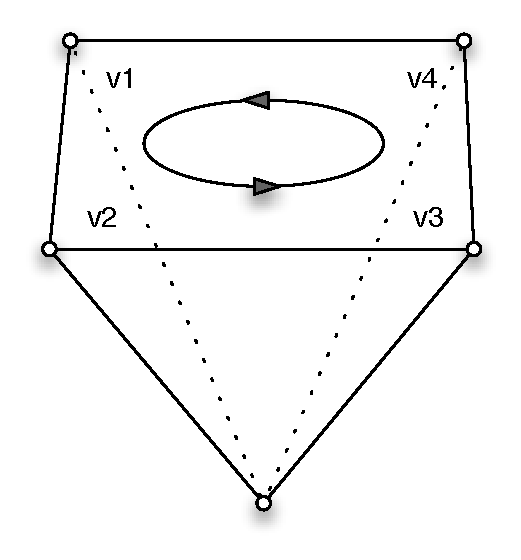
\includegraphics[scale=0.18]{../../../graphdod/counter.pdf}
   \end{center}
  \caption{}
\label{fig:counter}
\end{floatingfigure}


Each connected component $U$ has a solid angle $\sol(U)$, which
is defined to be the area of $U\cap S^2$.  The sum of the
solid angles is the area of $S^2$:
 $$
 \sum_{U\in[Y(G')]} \sol(U) = 4\pi.
 $$

If $U=U_F$ is a connected component and $v$ a vertex of $F$, then there
is an {\it azimuth angle} assigned to $(U,v)$ with the property
that if $F_1,\ldots,F_k$ are all the faces of $G(\Lambda)$
that contain $v$, the sum of the azimuth angles around
$v$ is $2\pi$:
  $$
  \sum_{i=1}^k \op{azim}(U_{F_i},v) = 2\pi.
  $$
Equivalently, 
the azimuth angle equals the interior angle of the spherical
polygon $U\cap S^2$ at $v/|v|$.  By Girard's formula for
the area of a triangle or polygon,  for
$F = (v_1,\ldots,v_r)$:
  $$
  \sol(U_F) + (r-2)\pi = \sum_{i=1}^k \op{azim}(U_F,v_i)
  $$
%When $\op{azim}(U_F,v) \ge \pi$, we say that $v$ is a concave
%vertex of $F$.  Otherwise, we say it is convex.

Set $\omega(\Lambda)=\op{vol}(\Omega_{trunc}(\Lambda,0))$.
If $U$ is a connected component of $Y(G')$, set
  $$\omega(\Lambda,U) = \op{vol}(U\cap \Omega_{trunc}(\Lambda,0)).$$
Then
  \begin{equation}\label{eqn:omegaU}
  \omega(\Lambda) = 
  \sum_{U\in[Y(G')]} \omega(\Lambda,U).
  \end{equation}
Set $M_{dod}=0.42755$ and set  $\mu(\Lambda)= \omega(\Lambda)- 4\pi M_{dod}$.
The desired inequality is then
that $\mu(\Lambda) > \mu(\Lambda_{dod})$.  
We have 
$$
  \mu(\Lambda_{dod}) \approx 0.177540.
$$
%%I don't use the term, to avoid conflicts with the terminology in \cite{DCG}.
The number $\mu(\Lambda_{dod})$ is called the {\it squander target} in \cite{arx}.  
When $U$ is a connected component of $Y(G')$, set
 \begin{equation}\label{eqn:mU}
  \mu(\Lambda,U)= \omega(\Lambda,U) - M_{dod} \sol(U).
  \end{equation}
Then
$$
\mu(\Lambda) = \sum_{U\in[Y(\Lambda)]} \mu(\Lambda,U).
$$




Now specialize again to the situation where $G'=G(\Lambda)$.
In this case, write $X(\Lambda)=X(G(\Lambda))$, $Y(\Lambda)=Y(G(\Lambda))$,
and so forth.
A connected component of $Y(\Lambda)$
is called a {\it standard component.}  (This term is a
reparametrization of a term by the same name
in the proof of the Kepler conjecture.)


If $U$ is indexed by a triangle $F=\{v_1,v_2,v_3\}$ in the graph,
then $U = \op{aff}_+^0(0,\{v_1,v_2,v_3\})$.  In this case,
$\omega(\Lambda,U)$ is precisely the volume of the region
already considered in Equation~\ref{eqn:omega-3}.

If $U$ is not indexed by a triangle, then
   $$\omega(\Lambda,U) = \op{vol}(U\cap\Omega_0(\Lambda,0)).$$
The formula for $\omega(\Lambda,U)$ in this case follows
by inclusion-exclusion as in Section~\ref{sec:in-ex}.  Suppose
that $F$ is a face of $G(\Lambda)$ whose vertices are given
by $(v_1,\ldots,v_r)$ (listed consecutively around the face).
Set $h_i=|v_i|/2$, $t=t_{dod}$, $b^\pm_{i}=\eta_V(0,v_i,v_{i\pm 1})$,
$\lambda=(1,0)$.
By \cite[Eqn.~7.12]{DCG}, inclusion-exclusion gives\FIXX{Double check.}
\begin{equation}\label{eqn:in-ex-U}
\begin{array}{lll}
\omega(\Lambda,U_F) &= \sol(U_F) \phi(t,t,\lambda) + \\
&\quad \sum_{i=1}^r (\azim(U_F,v_i) A(h_i,t,\lambda) - \quo(h_i,b_i^+,t) - 
\quo(h_i,b_i^-,t)).
\end{array}
\end{equation}
The derivation of this formula relies on two geometric facts.  First,
each quoin lies entirely in a single standard component.
Second, for each $1\le i\le r$, let $H_{\pm}$ be the open half-plane
bounded by the plane through $\{0,v_i,v_{i\pm 1}\}$, so
that $H_+\cap H_- \cap V = U_F\cap V$, for some neighborhood $V$ of $v$.
Then,   $C(v_i)\cap H_+\cap H_-\subset U_F$.
These facts are justified in \cite[Lemma~12.5]{DCG}.  The reparametrization
version appears in \cite{arx}.

Theorem~\ref{thm:main} shows that $\mu(\Lambda,U)$ is positive
for every standard component $U$.  The constant
$M_{dod}$ is chosen so that the minimum of $\mu(\Lambda,U)$ -- as
both $\Lambda$ and $U$  vary -- is very close to zero (about $10^{-7}$).
The function $\mu$ tends to have better numerical behavior
than $\omega$.  For that reason, even though the two
functions carry essentially the same information,
estimates are expressed in terms
of $\mu$ rather than $\omega$, whenever possible.

\begin{remark}\label{rem:sq} The function $\mu$ is closely related to a function
$\tau(\cdot,t)$ that is used in the proof of the Kepler conjecture.  The
function $\mu$ is, up to a small error term, a positive multiple
of $\tau(\cdot,t_{dod})$.   The small
error term comes from the fact that in this article, the constant
$M_{dod}$ is used, and in \cite{DCG} the constant
$M_0=1/(3 \delta_{tet})$ is used, where $\delta_{tet} = \sqrt8 \arctan(\sqrt2/5)$.  (The constant $\delta_{tet}\approx 0.7796$ is Rogers's famous bound on the density of sphere packings.)  The difference is small:
   $$M_0 - M_{dod} \approx 1.86 \times 10^{-7}.$$
Because of the close similarity between $\mu$ and $\tau(\cdot,t_0)$,
for every estimate involving $\tau(\cdot,t_0)$ there is apt to
be an analogous estimate involving $\mu$.  The translation involves
replacing $M_0$ with $M_{dod}$, $t_0$ with $t_{dod}$ and rescaling the
resulting function by an explicit positive scalar to get $\mu$.
%One other difference is that in general, 
%much weaker estimates are sufficient in the
%case of the Dodecahedral conjecture than in the solution to the
%sphere packing problem.
%To draw out the parallels between the two articles,  call
%an estimate in this article a $\mu$-$\tau$ analogy of an estimate
%in \cite{DCG} if this translation between functions applies.
\end{remark}



\section{The Main Estimate}

This section proves the main estimate, which gives a lower
bound on the function $\mu(\Lambda,U)$ for any standard component $U$.
The standing
assumptions on $\Lambda$ remain in effect: $0\in\Lambda= \Lambda(0,2t_{dod})$ and $G(\Lambda)$ is  biconnected.  This section makes
no assumptions on the cardinality 
of $\Lambda$ except where explicitly stated.

\begin{theorem}\label{thm:main}  
Let $\Lambda$ be a finite packing satisfying the
standing assumptions.  Let $U_F$ be a standard component indexed by
a face $F$ of $G(\Lambda)$.  Suppose that the polygon 
$F$ has $n$ vertices.  Then
   $\mu(\Lambda,U_F) > t_n$, where 
$$
\begin{array}{lll}
 t_3 &= 0\\
 t_4 &= 0.031\\
 t_5 &= 0.076\\
 t_6 &= 0.121\\
 t_7 &= 0.166\\
 t_n &= \mu(\Lambda_{dod}),\quad n\ge 8.
\end{array}
$$
\end{theorem}

The proof of this theorem is somewhat long.  The proof extends for 
twenty pages in  \cite[pp.19-38]{arx}.  The analogous estimate in
the proof of the Kepler conjecture takes a full thirty pages 
\cite[pp.126-156]{DCG}.
We cannot pretend to give justice to the proof under the page constraints
imposed on this version.  The reader is referred to the
two articles just cited for full details of the proof.  This article
 gives a general summary of the ideas of the proof, with 
references for the reader who wishes to pursue the proof in greater detail.

\subsection{verifications in low dimension}

The first two cases $n=3,4$ of the theorem can be handled directly with
interval arithmetic, because they are explicit nonlinear 
inequalities involving a small number of variables.  The case $n=3$ can
be expressed as a nonlinear optimization problem over a tetrahedron
whose edge lengths vary in length between $2$ and $2t_{dod}$.  In other
words, it is a minimization problem on the six-dimensional 
domain $[2,2t_{dod}]^6$. This is readily treated by interval arithmetic \cite[exact ref~XX]{code}

The case $n=4$ can also be directly proved with interval arithmetic.  
Here the optimization runs over a nine-dimensional domain.  The
quadrilateral face $F=(v_1,v_2,v_3,v_4)$ is parameterized up to rigid
motion by the nine variables (3 coordinates for each of four points
minus the 3 dimensional group of rotations).  Monotonicity arguments
reduce the configuration to a seven-dimensional domain.  (Two of the
points $v_i$ can be rescaled $v_i \mapsto \lambda v_i$ with $0 < \lambda \le 1$ until a constraint is met, 
because parallel shifts in faces of a truncated Voronoi cell towards the origin are decreasing in volume.)  The inequality $\mu(\Lambda,U)> t_4$ on
a seven-dimensional domain can be proved directly by interval arithmetic \cite[exact ref~XX]{code}.

\subsection{strategy: superadditivity}

% XX There are problems with the constants in version2.
% For instance, p22 says D_{dod}(3,2)=0.181, but page 20 gives D_{dod}(3,2)=0.0496.
% page22, (n,k)=(3,2) is incompatible with page 20. I am reverting to
% the treatment in version 1.
Define constants $D_{dod}(3,1) = 0.0161$ and $D_{dod}(n,k) = t_{n+k} - D_{dod}(3,1)k$,
for $n\ge 3$, $0\le k\le n$ and $n+k\ge 5$.  With these definitions,
when $n_1,n_2\ge 3$, $0\le k_1\le n_1$, $0\le k_2\le n_2$ and $n_1+k_1,n_2+k_2\ge 5$,  the following supperadditivity holds:
\begin{equation}\label{eqn:super}
  D_{dod}(n_1,k_1) + D_{dod}(n_2,k_2) \ge D_{dod}(n_1+n_2-2,k_1+k_2-2).
\end{equation}
In fact, this follows immediately from the definitions and the
easily verified inequality,
for $m,n\ge 5$,
$$
t_m + t_n \ge t_{m+n-4} + 2 D_{dod}(3,1).
$$
Note that there are only finitely many cases involved in the
verification of this identity,
because $t_n$ is constant for $n\ge 8$.


One of the basic strategies of the proof is to give a partial triangulation
of the face $F$ (with $n$ sides)
into smaller polygons $F_1,\ldots,F_r$.   The polygon
$F_i$ will have $n_i$ sides.  Let\footnote{More accurately,
$k_i$ is the number of edges $\{u,v\}$ of $F_i$ with $|u-v|\ge 2t_{dod}$.} 
$k_i$ be the number of edges
of $F_i$ that are not one of the original edges of $F$. 
Drawing a diagonal increases the number of oriented edges by
two, and this is the reason for the shift by two on the right
hand side of (\ref{eqn:super}).   The proof defines
a decomposition of $U_F$ into smaller components $U_i$ corresponding
to each $F_i$, gives a bound $\mu(\Lambda,U_i) > D_{dod}(n_i,k_i)$
and uses superadditivity (\ref{eqn:super}) to prove the identities:
\begin{equation}\label{eqn:mu}
  \mu(\Lambda,U_F) = \sum_{i=1}^r \mu(\Lambda,U_i).
\end{equation}
\begin{equation}\label{eqn:super-mu}
\sum_{i=1}^r \mu(\Lambda,U_i) > \sum_{i=1}^r D_{dod}(n_i,k_i)
 > D_{dod}(n,0) = t_n.
\end{equation}

The idea is that the objects $U_i$ are lower-dimensional objects
than $U_F$ (that is, the polygons  have fewer edges).
The dimension controls the complexity
of the estimates.  Thus a series of inequalities $\mu(\Lambda,U_i) > D_{dod}(n_i,k_i)$
can be expected to be easier to prove than a single inequality
$\mu(\Lambda,U_F) > t_n$ in higher dimension.  

On the other hand, if the edges of the polygons $F_i$ are allowed
to get too long, numerical experiments show that function $\mu(\Lambda,U_i)$
tends to become numerically unstable.  This prevents 
an overly aggressive  triangulation of $F$.
These experiments lead
 to a restriction of at most $3.2$ on the edge lengths.

A triple $(u,v,w)$ is called {\it unstable}
if $u,v,w$ are distinct vertices of $\Lambda^*$ such
that 
$$
|u| < 2t_{dod},\ |v| < 2 t_{dod},\ |u-v|< 2t_{dod},\  |v-w|< 2t_{dod},\ \text{and } |u-w|>\sqrt8.$$  
(The 
strict inequalities are significant in the arguments that follow.
In most places in the proof, one can be sloppy about whether
weak or strict inequalities are used, but not here.)
A pair $\{u,v\}$ is {\it unstable} if there exists $w$ such that $(u,w,v)$
is unstable.  Otherwise it is said to be {\it stable}.
Unstable edges $\{u,w\}$ create
 numerical instabilities and are best avoided.


\subsection{construction of subcomponents}\label{sec:sub}

Let $F$ be a face of the graph $G(\Lambda)$ and let $U_F$ be the
corresponding standard component.  Represent $F$ as a cycle
$(v_1,\ldots,v_n)$ with $v_i\in\Lambda^*$.  The function
$\mu(\Lambda,U_F)$ depends  on $\Lambda^*$ only through
$v_1,\ldots,v_n$.  Thus, for the purpose of the proof of
Theorem~\ref{thm:main},  assume without loss of generality
that $\Lambda^* = \{v_1,\ldots,v_n\}$.

Say that $u\in\Lambda^*$ is visible from $v\in\Lambda^*$ if
$\{0,u,v\}$ is not a collinear set and if
$\op{aff}_+^0(0,\{u,v\})\subset U_F$.  When this occurs, 
call the pair $\{u,v\}$ {\it internal}.  When $\{u,v\}$
is  internal, if the edge $\{u,v\}$ is added to the
graph $G(\Lambda)$, the graph continues to be spherical.

Define $\{u,v\}$ to be a {\it distinguished} pair in $U$ if
\begin{enumerate}
\item  $|u-v|\le3.2$, 
\item $\{u,v\}$ is internal.
\item  $\{u,v\}$ is stable.
\end{enumerate}  

Inductively, build a set $X$ of distinguished edges as follows.
Start with $X=\emptyset$.
Order the distinguished pairs $\{u,v\}$ by increasing
length $|u-v|$.  Considering each
distinguished edge $\{u,v\}$ in turn,
if it satisfies
the non-crossing condition
  $$
  \op{aff}_+^0(0,\{u,v\}) \cap \op{aff}_+^0(0,\{u',v'\}) = \emptyset,
  \text{ for } \{u',v'\}\in X,
$$
then add it to $X$, 



Let $G'(\Lambda)$ be the graph on vertex set $\Lambda^*=\{v_1,\ldots,v_n\}$ obtained by adding the edges $X$.  By the non-crossing
conditions, $G'(\Lambda)$ is a spherical graph.  
%By \cite[Lemma~4.15]{arx}
%(which is a reparametrization of Lemma~\ref{}), every
%internal edge $\{u,v\}$ of $U_F$ such that $|u-v|\le$
By the Jordan curve theorem for polygons, $Y(\Lambda)$ has two connected 
components,
$U_F$ and the complementary region $U_{F'}$.
Each
connected component $U'\subset Y(G')$ is either a subset of $U_F$ or $U_{F'}$.
Since all the added edges are internal to $U_F$, there is exactly
one component of $Y(G')$ that lies in $U_{F'}$, and that component
is equal to $U_{F'}$.  Write $[Y(G')]^* = [Y(G')]\setminus\{U_{F'}\}$
for the set of components of $Y(G')$ internal to $U_F$.

Enumerate them $U_1,\ldots,U_r$.  Define $\omega(\Lambda,U_i)$ and
$\mu(\Lambda,U_i)$, as usual,  by (\ref{eqn:mU}).  Then
(\ref{eqn:in-ex-U}) and (\ref{eqn:mu}) hold.  In fact, the justification
given for (\ref{eqn:in-ex-U}) holds verbatim in this more general
context. Let $n_i$ be the number of edges of the face
$F_i$ of $G'$ corresponding to $U_i$.  Let $k_i$ be the number of edges
$\{u,v\}$
of $F_i$ such that $|u-v|\ge 2t_{dod}$. (These are edges of $G'$ that do not
belong to $G(\Lambda)$ and edges of $G(\Lambda)$ that have
length exactly $2t_{dod}$.)  

The function $\mu(\Lambda,U_i)$ depends on $\Lambda$ only through
the vertices of $\Lambda$ on $F_i$.  Thus, for purposes of estimating
$\mu(\Lambda,U_i)$ for fixed $i$,  assume that $\Lambda$
is equal to the set of vertices of $F_i$.  The estimates can then
be expressed locally.
   This motivates the following definition.

\begin{definition}
Let $\Lambda$ be a packing such that $0\in\Lambda=\Lambda(0,2t_{dod})$.  
Let $G$ be a graph on vertex set $\Lambda^*$ 
consisting
of a single cycle containing $n\ge 3$ vertices.  
Suppose that $G$ is spherical. 
Let $U\in [Y(G)]$ be a connected component of $Y(G)$.  
The triple $(\Lambda,G,U)$ is called a {\it local configuration} if the
following conditions hold:
\begin{enumerate}
\item Every edge $\{u,v\}$ of $G'$ satisfies $|u-v|\le 3.2$.
\item If
$\{u,v\}$ is internal in  $U$, then $|u-v|\ge \sqrt8$.
\item If $\{u,v\}$ is internal in $U$ and stable,
then $|u-v|\ge 3.2$.
\end{enumerate}
\end{definition}

% Do we need a hypothesis that keeps the region from being exchanged with
%its complement on triangles, quadrilaterals, etc.? I don't think so.

Let $n=n(\Lambda,G,U)$ be the cardinality of $\Lambda^*$.  Equivalently,
$n$ is the number of edges in the graph $G$.  Let
$k=k(\Lambda,G,U)\le n$ be the number of edges $\{u,v\}$ of $G$ such
that $|u-v|\ge 2t_{dod}$. 

The main estimate (Theorem~\ref{thm:main}) now follows from the following
refined version of the estimate and superadditivity.

\begin{theorem}\label{thm:main'}  
Let $(\Lambda,G,U)$ be any local configuration.
Let $n=n(\Lambda,G,U)$ and $k=k(\Lambda,G,U)$ be the corresponding constants.
Assume that $n+k\ge 4$.  Then
   $$
   \mu(\Lambda,U) > D_{dod}(n,k).
   $$
\end{theorem}

\subsection{deformations}


The proof of Theorem~\ref{thm:main'} is a total induction argument
on  the cardinality $n$ of $\Lambda^*$.  The induction base case
is vacuous, if the induction starts at $n=2$, since every
local configuration has $n\ge 3$.
Take $n\ge 3$ and assume that
Theorem~\ref{thm:main'} holds for any local configuration with
cardinality less than $n$.  

The strategy of the proof is to deform the local configuration $(\Lambda,G,U)$ by moving a single vertex $v\in\Lambda^*$ at a time in a way
that preserves the constraint of being a local configuration,
preserves $n$, 
is non-increasing in $\mu(\Lambda,U)$, 
and is non-decreasing in $D_{dod}(n,k)$.
Under these conditions, any counterexample to the theorem propagates 
to a new counterexample under the deformation.
Note that it is easily checked that $D_{dod}(n,k) \le D_{dod}(n,k+1)$, for all
$n\ge 3$ and all $n> k\ge0$.  Thus, the condition that $D_{dod}(n,k)$
is non-decreasing can be replaced with the constraint that $k$
is non-decreasing under deformation.

The azimuth angle
$\op{azim}(U,v)$ is defined for each $v\in\Lambda^*$.  
Call $v$ {\it concave} in $U$
if $\op{azim}(U,v)\ge\pi$.  Otherwise, say that $v$ is convex
in $U$.  If every vertex $v$ is convex in $U$, then $U$
is a convex set.  When $U$ is convex, it is known that $U$
is contained in some open half-space whose bounding plane
contains the origin.  Moreover,
if $U$ is convex (and $n\ge 3$),
it is known that $u$ is visible from $v$ in $U$
for any two nonadjacent vertices $u,v\in\Lambda^*$.  Note that when $U$ is 
convex, the conditions on local configurations require that
$|u-v|\ge\sqrt8$, for any two non-adjacent vertices $u,v\in\Lambda^*$,
because $\{u,v\}$ is automatically internal.

\subsection{deformation at concave vertices}\label{sec:concave}

The most challenging part  of Theorem~\ref{thm:main'} is the
proof when the local configuration has a concave vertex.  This subsection
sketches the proof in that case.

The following subsections describe several different  deformations.  For each,
we describe the deformation, the starting and halting conditions on 
the deformation.  We show that the $(\Lambda,G,U)$ remains a local
configuration throughout the deformation, 
 that  $\mu(\Lambda,U)$ in non-increasing, and $k$ is
non-decreasing.


Let $v$ be concave in $U$.  Let $u,w$ be the two vertices of
$\Lambda^*$ adjacent to $v$ in $G$. 
If $|v-u|=|v-w|$, then the deformation is defined as the continuous motion
of $v$ preserving $|v|$,  moving along the bisecting plane of $\{u,w\}$
and increasing $|v-u|$.  If $|v-u|<|v-w|$, then the deformation
is defined as the continuous motion of $v$ preserving $|v|$ and
$|v-w|$ and increasing $|v-u|$.

The deformation must halt if any of the following conditions
are met.  (If the initial configuration satisfies any of these conditions,
no deformation at $v$ occurs.)
\begin{enumerate}\label{e:halt}
\item For some $v'\in\Lambda^*\setminus\{u,v,w\}$, 
$\{v,v'\}$ is internal and $|v-v'|\le \sqrt8$.
\item For some $v'\in\Lambda^*\setminus\{u,v,w\}$,
$\{v,v'\}$ is internal, stable, and $|v-v'|\le 3.2$.
\item $|v|\ge 2.2$ and $|u-v|=|v-w|=3.2$.  
\item $|v|< 2.2$, 
and $|u-v|\ge 3.07$, $|v-w|\ge 3.07$.
\end{enumerate}
%% I think it is better to use the constant 3.07-t_{dod}. This is done below.

By a calculation of derivatives with interval arithmetic,
the deformation is non-increasing in $\mu(\Lambda,U)$ \cite[Lemma~7.7]{arx}.  (Although, the function $\mu(\Lambda,U)$ is potentially a 
function of a large number of variables, the derivative of $\mu$
along the deformation depends only on the six edge lengths  of
the simplex $\{0,u,v,w\}$.  This derivative calculation is within
the reach of interval methods.)
The deformation is non-decreasing in $k$, because the length
$|v-u|$ is increasing.

The deformation preserves $|v|$,
so that the constraint $0\in\Lambda=\Lambda(0,2t_{dod})$ is preserved.
For $\Lambda$ to remain a packing,  the condition
 $|u-v|\ge 2$, for $u,v\in \Lambda$ must hold.
This article does not repeat the rather technical proof that
the condition
 $|u-v|\ge 2$ is preserved, for $u,v\in\Lambda^*$.  The proof
runs a couple  of pages \cite[Lemma~7.6]{arx}.
It is the reparametrization of \cite[Lemma~12.20]{DCG}.

The next constraint is that the deformation should preserve the condition
that $G$ is spherical.  
If not, then the deformation produces
a situation where $v\in \op{aff}_+(0,\{u_1,u_2\})$ for some fixed edge $\{u_1,u_2\}$
of $G$; or $u_1\in \op{aff}_+^0(0,\{v,u\})$ for some fixed $u_1$ of $\Lambda^*$.
The first case is ruled out by \cite[Remark~p.22]{arx}, which is the reparametrization of \cite[\S12.7,p.132]{DCG}.  The second case is ruled out by 
the argument of \cite[p.27]{arx}, a reparametrization of 
\cite[\S12.8,p.134]{DCG}.

The cardinality $n$ of the vertex set $\Lambda^*$ is preserved.
The set of edges of the graph of $G$ is combinatorially determined and
remains fixed under deformation.  In particular, $G$ remains a single
cycle.  Since $G$ is spherical and consists of a single
cycle, the set $Y(G)$ has two connected components throughout the
deformation.  The component $U$ evolves continuously under deformation.   

The condition for a pair $\{v_1,v_2\}$ to be
internal is not constant under deformation.  Nevertheless,
\cite[p.23]{arx} (or \cite[p.132]{DCG}) 
shows that a pair $\{v_1,v_2\}$
cannot switch to internal when $|v_1-v_2| \le \sqrt8$.  When $\{v_1,v_2\}$ is stable,
it cannot switch to internal when $|v_1-v_2|\le 3.2$. 
The enumerated conditions on the
internal pairs $\{v_1,v_2\}$ in the definition of local configurations
now follow from the halting conditions. (In fact, the halting conditions on internal edges
can be replaced with equality, because of the
constraints on local configurations.)

The preceding arguments fully justify that the deformation preserves
the property of being a local configuration, and that
any counterexample to the lemma is propagated under
the deformation.


There is no loss in generality to assume that the first two halting conditions are never
met.  Indeed, these conditions allow a new stable internal edge $\{v,v'\}$ to be formed.  The
graph $G$ can be extended to a spherical graph $G'$ by adding the internal edge.
The component $U$ is partitioned into a disjoint union of two components $U_1,U_2$ 
of $Y(G')$ and the separating set $\op{aff}_+^0(0,\{v,v'\})$.  The vertex set
$\Lambda$ is the union of $\Lambda_1\cup\Lambda_2$ with $\Lambda_1\cap\Lambda_2=\{0,v,v'\}$
with corresponding cycles $G_1$ and $G_2$.  Both $(\Lambda_1,G_1,U_1)$ and $(\Lambda_2,G_2,U_2)$ are local configurations.  Moreover, $\mu(\Lambda,U) = \mu(\Lambda_1,U_1)+\mu(\Lambda_2,U_2)$.  By the induction hypothesis and superadditivity, the theorem follows in this case.
As the proof in this case now complete, the following arguments
assume that the first two halting conditions are never met.

Thus, the halting condition on $v$ simplifies to 
\begin{equation}\label{eqn:halt}
\begin{cases}
|u-v|=|v-w|=3.2,& \text{when } |v|\ge 2.2\\
%|u-v|=|v-w|=3.2,& \text{when } v \text{ is the only concave vertex of } U,\\
|u-v|\ge 3.07, |v-w|\ge 3.07,& \text{otherwise.}
\end{cases}
%\item $v$ is the only concave vertex of $U$, and $|u-v|=|v-w|=3.2$.  
%\item $|v|< 2.2$, $v$ is not the only concave vertex of $U$,
%and $|u-v|\ge 3.07$, $|v-w|\ge 3.07$.
\end{equation}
After repeating the deformation at all concave vertices, assume that the halting condition
holds for each concave vertex.  Note that the halting
condition at $v$ is incompatible with the length conditions in
the definition of an unstable triple $(v,w_1,w_2)$.  It
follows that every internal edge $\{u,w\}$
at a concave vertex $u$ is stable.  By the definition of local configuration, this
implies that $|u-w|\ge 3.2$.  Thus, the hypotheses in the following lemma are fulfilled.

\begin{lemma}\label{lemma:concave}  
Let $(\Lambda,G,U)$ be a local configuration with at least one
concave vertex.  Suppose that 
condition (\ref{eqn:halt}) holds at each concave vertex.  Suppose further at each internal
pair $\{u,v\}$ with $v\in\Lambda^*$ concave and $u\in\Lambda^*$ not adjacent to $v$,
that $|u-v|\ge 3.2$ holds.   Let $n,k$ be the parameters attached
to $(\Lambda,G,U)$.  Finally, assume the induction hypothesis that Theorem~\ref{thm:main'}
holds for all $n'<n$. Then
   $$\mu(\Lambda,U) > D_{dod}(n,k).$$
\end{lemma}

\begin{proof} (Sketch)  By definitions,
$\mu(\Lambda_{dod}) = t_8 \ge t_{n+k} - D_{dod}(3,1)k = D_{dod}(n,k)$, so it is
enough to prove $\mu(\Lambda,U) > \mu(\Lambda_{dod})$. 
Define $\psi(v,\lambda)$ to be the angle of a triangle with sides $|v|,\lambda,t_{dod}$
opposite the side $\lambda$.  Recall the right-circular cone 
$\op{rcone}(0,v,\cos\psi(v,\lambda))$ from the discussion of Tarski arithmetic.
The proof breaks into two
cases: there are at least two concave vertices, and there is exactly one concave vertex.

Suppose that there are at least two concave vertices.  Pick two $v_1,v_2$.
Partition $U$ into three
components $U_i = U\cap \op{rcone}(0,v_i,\cos\psi(v_i,3.07/2))$, for $i=1,2$; and
$U_0= U\setminus (U_1\cup U_2)$.  It is known that
$U_1$ is disjoint from $U_2$ \cite[Lemma~3.7]{arx}.   A careful study of the geometry
of $U_1$ and $U_2$ shows the shape of $\Omega_{trunc}(\Lambda,0)\cap U_i$ and the
solid angle of $U_i$ depend only
on two parameters: $|v_i|$ and $\op{azim}(U,v_i)$.  Interval arithmetic gives
the estimates
  $$\mu(\Lambda,U_i) \ge \mu(\Lambda_{dod})/2,\quad i=1,2$$
for these two-dimensional objects \cite[\S7.2.6]{arx}.  On the remaining piece, $\mu(\Lambda,U_0)>0$ holds
\cite[p.138]{DCG}.  The sum of these terms is
  $$
  \mu(\Lambda,U) = \sum_{i=1}^3 \mu(\Lambda,U_i) > \mu(\Lambda_{dod}).
  $$

Now suppose that there is exactly one concave vertex $v$.  In this case, if $u\in\Lambda^*\setminus\{v\}$
is not adjacent to $v$, then $\{u,v\}$ is internal \cite[p.140]{DCG}.  This implies
that $|u-v|\ge 3.07$ for all $u\in\Lambda^*\setminus\{v\}$.
Consider the deformation that rescales $v$ to decrease its norm $v\mapsto s v$, for 
$2/|v|\le s\le 1$. Under this deformation, $\Omega_{trunc}(\Lambda,0)\cap U$ decreases
in volume and the solid angle is unchanged, so that $\mu(\Lambda,U)$ decreases.
Combine this deformation with the deformation given above so that the
constraints in the hypothesis of the lemma are preserved.  As before, the induction
hypothesis is used to avoid the first two conditions of (\ref{e:halt}).
The constants $n,k$ are unchanged; $\Lambda$ remains a packing, and so forth.
The deformation continues\footnote{A typo in \cite{arx}  incorrectly states $|v|=2$.} until the halting condition $|v|\le 2.2$ is satisfied. 

Let $U_1 = U\cap \op{rcone}(0,v,\cos\psi(v,3.07-t_{dod}))$ and $U_0 = U
\setminus U_1$.  A study of the geometry of $\Omega_{trunc}(\Lambda,0)
\cap U_1$ shows that its volume and solid angle only depend 
on two parameters $|v|$ and
$\op{azim}(U_1,v)$.  An interval arithmetic calculation over this
two-dimensional space, using $|v|\le 2.2$, gives
$$
\mu(\Lambda,U_1) > \mu(\Lambda_{dod}).
$$
(See \cite[\S7.2.6]{arx}. The constant there 1.94159 is a typo.
It should be $3.07-t_{dod}$.  The typo does not affect the proof.)
The inequality $\mu(\Lambda,U_0)>0$ holds for the same reason provided
in the case of two convex vertices.  This completes
the proof of Lemma~\ref{lemma:concave}.
% XX Recheck the calculation of 7.2.6 to see the typo does no harm.
\end{proof}


\subsection{deformation at convex vertices}

The results of the previous subsection
reduce the proof of Theorem~\ref{thm:main'} to
the case where $U$ is convex at every vertex.  A convex
spherical polygon on a unit sphere has perimeter
at most $2\pi$.  A polygon $F$ in $G(\Lambda)$ projects to
a spherical polygon on the unit sphere $S^2$.  An edge $\{u,v\}$ of
$F$ satisfies bounds $|u|,|v|\in[2,2t_{dod}]$, $|u-v|\ge 2$. This
implies that every edge of the spherical polygon has arc length
at least $\theta=2\arcsin(1/(2t_{dod}))$, and that the number
of edges is at most seven ($2\pi/\theta < 8$).

In this subsection, the geometry is much more explicit than in the
previous subsection, because $U$ is convex and $F$ has at most seven sides.
Let $(G,\Lambda,U)$ be a local configuration.
Let $(n,k)$ be the associated parameters.
This section gives the proof of Theorem~\ref{thm:main'} under 
the total induction hypothesis on $n$ and assuming the truth
for local configurations with parameter $n$ and a concave vertex.
The method, again, is to produce a deformation of the local
configuration by moving one vertex $v$ at a time.



Let $(\Lambda,G,U)$ be a local configuration with $U$ convex.
Let $v\in\Lambda^*$.  
Let $u,w$ be the two vertices of $\Lambda^*$
adjacent to $v$.  By convexity, every pair $\{u,v'\}$,
with $v'\in\Lambda^*\setminus\{u,v,w\}$, is internal.


\subsubsection{first convex deformation}

Consider the deformation that fixes $|v|$ and $|v-w|$ and
moves $v$ to decrease $|v-u|$.  
The deformation halts (or never starts) once any
of the following conditions holds.
\begin{enumerate}\label{e:halt-convex}
\item For some $v'\in\Lambda^*\setminus\{u,v,w\}$, 
$\{v,v'\}$, $|v-v'|\le \sqrt8$.
\item For some $v'\in\Lambda^*\setminus\{u,v,w\}$,
$\{v,v'\}$ is  stable, and $|v-v'|\le 3.2$.
\item $\op{azim}(U,v)\ge\pi$.
\item There exists $v'\ne v$ such that 
$(u,v',w)$ is an unstable triple and $|u-w|\le3.2$.
\item $|v-u|=\sqrt8$.
\item $|v-u|=2t_{dod}$.
\item $|v-u|=2$.
\end{enumerate}
%% I'm not sure what role the sqrt8 plays in this proof.
% I believe that 

As with deformations at nonconvex vertices, 
the deformation of a local
configuration remains a local configuration.  Here, in the
convex situation, the proof is more elementary, because the
geometry is explicit.  For instance, the condition that
$\Lambda$ remains a packing follows immediately from the halting
conditions, because every nonadjacent vertex gives an internal
edge.

The function $\mu(\Lambda,U)$ is non-increasing under the
deformation by \cite[Lemma~7.8]{arx}.  The value of
$k$ in non-decreasing by the halting conditions. 

\subsubsection{second convex deformation}

Let $(\Lambda,G,U)$ be a local configuration with $U$ convex.
Consider the deformation that fixes $|u-v|$ and $|u-w|$ and
moves $v$ to increase or decrease $|v|$.  The direction
of the deformation is chosen to decrease $\mu(\Lambda,U)$.
The deformation halts (or never starts) once any
of the following conditions holds.
\begin{enumerate}\label{e:halt-convex2}
\item For some $v'\in\Lambda^*\setminus\{u,v,w\}$, 
$\{v,v'\}$, $|v-v'|\le \sqrt8$.
\item For some $v'\in\Lambda^*\setminus\{u,v,w\}$,
$\{v,v'\}$ is  stable, and $|v-v'|\le 3.2$.
\item $\op{azim}(U,v)\ge\pi$.
\item $|u-v|\ne 2,2t_{dod},\sqrt8$.
\item $|u-w|\ne 2,2t_{dod},\sqrt8$.
\item $|v|=2$.
\item $|v|=2t_0$.
\end{enumerate}

By an interval arithmetic calculation of derivatives,
the function $\mu(\Lambda,U)$ does not have a local
minimum, provided none of the halting conditions hold
\cite[Lemma~7.10]{arx}.  That is, the deformation can always continue
to decrease $\mu(\Lambda,U)$ until a halting condition is met.



\subsubsection{completion of the proof}


\begin{proof} (Sketch)
With these two deformations at hand, the proof
of Theorem~\ref{thm:main'} can be completed.  Let $n$ be
the cardinality of $\Lambda^*$.
If $n=3$, the inequality of the theorem is an inequality
in six variables and can be verified directly by interval
arithmetic \cite{code}, \cite[\S7.4.1]{arx}.  Now assume
that $n>3$.  Furthermore, by previous estimates, $n\le 7$.


By induction, it may be assumed that
the theorem is established for all $n'<n$.  By previous arguments,
it may be assumed that the theorem is known for $U$ with a concave
$v$ (and the same value of $n$).

By the induction argument and the reduction to the convex case,
there is no loss in generality to assume that the first three
halting conditions (for both deformations) never occur.  

The  halting condition (4) is rather strange:
There exists $v'\ne v$ such that 
$(u,v',w)$ is an unstable triple and $|u-w|<3.2$.
(It was needed in the interval arithmetic verifications
that prove the monotonicity of $\mu(\Lambda,U)$.)  Note
that $v$ and $v'$ are both adjacent to $u,w$ when this
halting condition holds.  This implies that $n=4$.  

Consider the case $n=4$.  The dimension of a general configuration
is nine, parameterized by four lengths $|v|$ for $v\in\Lambda^*$,
four lengths $|u-v|$ for edges $\{u,v\}$ of $G(\Lambda)$, and $|u-v|$
for one internal pair $\{u,v\}$.
Even
if this halting condition becomes binding at $v$, deformations
can continue at the three other vertices, until some halting
condition holds at each vertex.  Eventually the deformations
reduce the dimension of the configuration to at most three.
Interval arithmetic finishes this case off \cite[\S7.4.2]{arx}.

With the case $n=4$ out of the way, the
the halting condition for the first convex deformation
reduces to
  $$
  |u-v| = 2, 2t_{dod}, \text{ or } \sqrt8.
  $$
The first convex deformation can be applied at each vertex 
so that this condition holds for every edge $\{u,v\}$ of $G(\Lambda)$.
Then, the halting conditions (4) and (5) of the second convex
deformation now never occur.  The second convex deformation can
be applied until $|v|=2$ or $|v|=2t_{dod}$ for each $v\in\Lambda^*$.

The local configuration $(\Lambda,G,U)$ is now a low-dimensional
object.  The only remaining continuous parameters are the lengths of
$(n-3)$ internal pairs $\{u,v\}$ needed to triangulate the
$n$-gon $G(\Lambda)$.  Thus, it has dimension $m=n-3$,
for $5\le n\le 7$.

Unfortunately, the proof does not end here with a simple interval
arithmetic calculation in low dimension.  It does not end
here because there is no control on the
lengths of the triangulating diagonals, and without any such
control the calculations are simply too numerically unstable.


A different strategy completes the proof, based on truncated
corner cells.  Although the dimension of this problem is now small,
this argument requires several pages.
See \cite[pp.30-38]{arx}.  It is modeled on a published
$14$-page argument in the solution to the sphere packing problem
\cite[\S\S13.2-13.11]{DCG}, following the same strategy.
Here is a brief summary of the two principal  methods that are used.

\textbf {Dealing with unstable edges:}  
If $(u,v,w)$ is an unstable triple, then the
halting conditions force $|u|=|v|=|u-v|=|v-w|=2$.  (This
relies on the strictness of the inequalities defining stability.)
The value of $|v|$ can be $2$ or $2t_{dod}$. In this final
stage of the proof, contrary to the constraints of Section~\ref{sec:sub}
on distinguished pairs,
it is now permitted to split the region $U$ into two pieces
$U_F,U_{F'}$ separated by $\op{aff}_+^0(0,\{v,w\})$, where
the pair $\{v,w\}$ is unstable and $|v-w|\le 3.2$.  
One of these pieces is indexed
by a triangle $F$.  Because of instability, the usual inequality
$\mu(\Lambda,U_F)> D_{dod}(3,1)$ does not hold.  To compensate,
stronger inequalities are proved for $\mu(\Lambda,U_{F'})$.
The deformations can continue on the component $U_{F'}$. Nevertheless,
it must be remembered that the induction hypothesis and the 
reduction to the convex case do not cover the stronger 
inequality for $\mu(\Lambda,U_{F'})$ that is now needed.

\textbf {Truncated corner cells:}  If $U$ has no unstable
internal $\{u,v\}$, then the following argument gives the
desired bound.  The component $U$ is partitioned into $n+1$
parts, one $U_v$ for each vertex $v\in\Lambda^*$ and a final part
for the remainder $U_0 = U\setminus(\cup_{v\in\Lambda^*} U_v)$.
The function $\mu(\Lambda,U)$ is a sum of terms $\mu(\Lambda,U_v)$
and $\mu(\Lambda,U_0) >0$.  The function $\mu(\Lambda,U_v)$
is a function of the six edges of $\{0,v,u,w\}$ (with $u,w$
adjacent to $v$) and most of these edges are fixed in length
by the deformations.  So the function $\mu(\Lambda,U_v)$
is readily bounded with interval arithmetic.  Each part
$$\Omega_{trunc}(\Lambda,0)\cap U_v$$
is called a {\it truncated corner cell}.  The defining conditions
for $U_v$ are
  $$
  U_v = U \cap \op{rcone}(0,v,\cos\psi(v,1.6)) \cap H(0,v,u) \cap H(0,v,w),
  $$
where $\psi(v,\lambda)$ is the angle defined in Section~\ref{sec:concave},
and $H(0,v,v')$ is the open half space containing $v$, bounded by
the plane through $0$ and through the circumcenter
of $\{0,v,v'\}$, orthogonal to the plane of $\{0,v,v'\}$.  The
sets $U_v$, as $v$ ranges over $\Lambda^*$, are disjoint from one
another.


%\textbf {Geometric impossibilities:}  Geometric arguments
%eliminate certainedge length combinations
%in the end game of the proof.  For example, if deformations
%produce the constraints
%  $$
%  |v|=2t_0,\ |v|=|w|=|u-v|=|v-w|=2,\ 
%  $$
%then the simplex $\{0,u,v,w\}$ has a single free parameter $|u-w|$.
%The largest value of $|u-w|$ occurs when the simplex flattens out
%into a planar arrangement.  A calculation gives $|u-w|< 3.2$.
%This gives an unstable pair $\{u,w\}$ along which $U$ can
%be separated.



We refer the reader to the unabridged version of the proof for details.
\end{proof}



\section{Classification of Tame Hypermaps}

This section turns to the problem of classifying a large finite collection
of planar graphs. For combinatorial simplicity, this classification is phrased
in terms of hypermaps, which are defined in the first subsection.
The next subsection shows how a sphere packing $\Lambda$ gives a hypermap.
The rest of the section is devoted to the classification problem.
A final subsection shows how a counterexample $\Lambda$ to the Dodecahedral
conjecture gives one of the hypermaps classified in this section.

\subsection{hypermap}

A hypermap is a tuple $(D,e,n,f)$, where $D$ is a finite
set, and $e,n,f$ are three permutations on that set that
compose to the identity:
$e\circ n\circ f = I$.  The elements of $D$ are called darts.
The permutations $e,n,f$ are called the edge permutation,
node permutation, and face permutation, respectively.
(A hypermap was previously defined as a finite set $D$ with
two permutations $f,n$, which amounts to the same thing,
since $e$ is uniquely determined by $f,n$.)

If $m$ is any permutation on $D$, write $D/m$ for the
set of orbits in $D$ under $m$.  Similarly, if $G$ is any
group of permutations on $D$, write $D/G$ for the set
of orbits of $D$ under $G$.  In particular, $D/\tangle{e,n,f}$
is the set of orbits under the group generated by $e,n,f$.
An orbit of $D$ under $f$ ($n$, or $e$) is called a face (resp.
node, or edge).

A planar graph gives  a hypermap
by the following procedure.  Starting with a planar graph,
place a dart at each angle.  That is, at a vertex of degree $k$,
place $k$ darts, one between each consecutive pair of edges.
The face permutation has a cycle for
each face of the planar graph and  traverses the
darts in a counterclockwise direction around each face.
The node permutation has a cycle for each vertex and traverses
the darts in a counterclockwise direction around each vertex.
The edge permutation is defined by the relation $e\circ n\circ f=I$.
It can be interpreted as an involution that pairs a dart next
to one endpoint of an edge with a dart at the other endpoint.
See Figure~\ref{fig:hypermap}.

% XX Draw figure hypermap of planar graph
\begin{floatingfigure}{80mm}
  \begin{center}
  %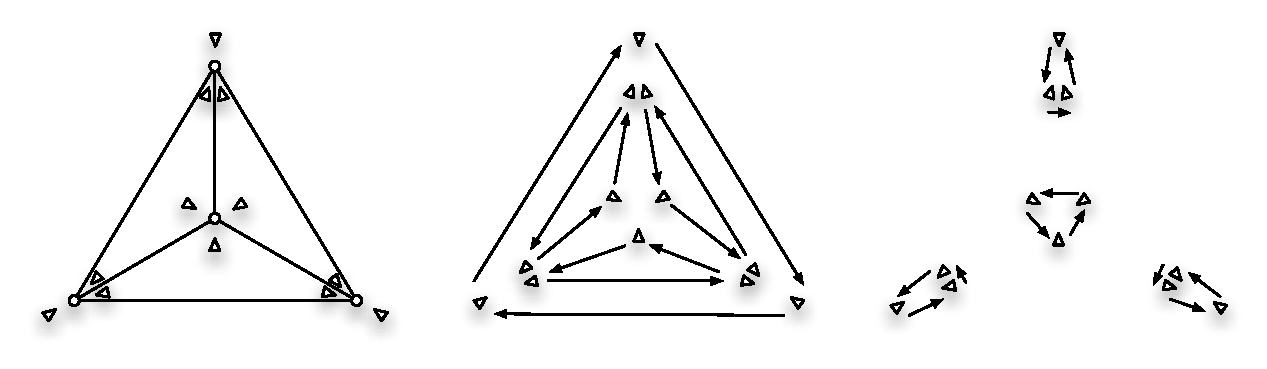
\includegraphics[scale=0.18]{../../../graphdod/hyper.pdf}
   \end{center}
  \caption{}
\label{fig:hypermap}
\end{floatingfigure}

Hypermaps are the primary combinatorial object used by Gonthier
in the formalization of the Four-Color theorem in COQ~\cite{Gon}.
Hypermaps, by being purely combinatorial, are more convenient
to represent on a computer than planar graphs.  


Not all hypermaps arise from a planar graph in this way.
Those that do have two special properties.  They are involutive
and planar in the following sense.   The definition
of planar hypermap is the standard condition on the Euler
characteristic, translated into the language of hypermaps.

\begin{definition}\label{def:involutive}
\mbox{}
\begin{itemize}
\item The hypermap $(D,e,n,f)$ is involutive, if $e$ is an involution:
$$
 e^2 = I.
$$
\item The hypermap $(D,e,n,f)$ is planar, if
   $$
   \#(D/e) + \#(D/n) + \#(D/f) = \# D + 2\#(D/\tangle{e,n,f}).
   $$
where $\# X$ denotes the cardinality of $X$.
\end{itemize}
\end{definition}

\subsection{packings and hypermaps}\label{sec:ph}

Let $\Lambda$ be a packing satisfying $0\in\Lambda=\Lambda(0,2t_{dod})$.  The graph
$G(\Lambda)$ is planar.   Assume that $G(\Lambda)$ is biconnected. 
This subsection describes in greater detail the
hypermap $H(\Lambda)$ attached to $G(\Lambda)$.

For each $v\in \Lambda^*$, let 
  $$E(v) = \{u \mid \{v,u\} \text{ is an edge in the graph } G(\Lambda)\}.$$
For each $u\in E(v)$, there is a half-plane $A(v,u)$ containing $u$, bounded by
the line through $\{0,v\}$.  There is a cyclic order on the half-planes $A(v,u)$,
moving in a counterclockwise circle around the ray emanating from $0$ through $v$.
Write $\sigma_v$ for the cyclic permutation on $E(v)$, given by this ordering.

Define the set of darts by
$$
D = \{(0,v,u,\sigma_v u) \mid u\in E(v)\}.
$$
Define face, edge, and node permutations on $D$ by
$$
\begin{array}{lll}
  f(0,v,w,u) &= (0,w,\sigma_w^{-1} v,v),\\
  e(0,v,w,u) &= (0,w,v,\sigma_w v),\\
  n(0,v,w,u) &= (0,v,u,\sigma_v u).
\end{array}
$$
A formal calculation shows that $(D,e,n,f)$ is an involutive hypermap.

The nodes of $(D,e,n,f)$ are in bijection with $\Lambda^*$ under the correspondence:
$$
  (0,v,w,u) \mapsto v\in\Lambda^*.
$$
The edges of $(D,e,n,f)$ are in bijection with the edges of $G(\Lambda)$ under the
correspondence:
$$
  (0,v,w,u) \mapsto \{v,w\}.
$$
The faces of $(D,e,n,f)$ are in bijection with the faces of $G(\Lambda)$ under the
correspondence:
$$
  x = (0,v,w,u) \mapsto ((f^{-1}x)_3,x_3,(f x)_3,(f^2 x)_3,\ldots),
$$
where $y_3$ is the third component of the four-tuple $y$ and each face is represented
as usual as cycle $(v_1,\ldots,v_n)$.
The set of darts is in bijection with the set of oriented edges of $G(\Lambda)$ under
the correspondence:
$$
(0,v,w,u)\mapsto (v,w).
$$
The graph $G(\Lambda)$ is connected.  This implies that $\tangle{e,n,f}$ acts
transitively on $D$.

The graph $G(\Lambda)$ is planar.  If $V,E,F$ are the number of vertices, edges,
and faces, then $V-E+F=2$; or equivalently, $V+E+F = 2 + 2E$.
Under the bijections just described, this implies that the cardinalities
of these sets satisfy
$$
     \#(D/e) + \#(D/n) + \#(D/f) = \# D + 2\#(D/\tangle{e,n,f}).
$$
Thus, the hypermap $(D,e,n,f)$ is planar.

\begin{remark}
In \cite{arx}, the basic combinatorial structure is called a {\it planar map} rather
than hypermap.  In that article, the combinatorial structure is represented in
computer code as a finite set of faces
 $$
  \{F_1,F_2,\ldots,F_r\},
 $$
and each face is represented as a cycle $(v_1,\ldots,v_n)$ of vertices.  This is
essentially equivalent to a hypermap.  This representation
is converted to a hypermap by sending $(v_1,v_2,\ldots,v_n)$ to the dart
$(0,v_1,v_2,\sigma_{v_1} v_2)$.  There are $n$-choices of which vertex $v_i$ to list
first in the cycle, and by taking all choices, $n$ darts are obtained.  Running
through all faces in this way, all darts are constructed.  In the opposite direction,
an earlier argument describes how a face of the hypermap gives a face of $G(\Lambda)$,
expressed as a cycle.
\end{remark}

\subsection{tameness}

This subsection defines a collection of hypermaps called tame Voronoi hypermaps.
The classification of these hypermaps, up to isomorphism, is one of the main steps
of the proof of the Dodecahedral conjecture.

Let $H=(D,e,n,f)$ be a hypermap.  A face of $H$ (that is, an orbit
of $D$ under $f$) is said to be a triangle, quadrilateral, pentagon, etc. if the cardinality
of the orbit is $3$, $4$, $5$, respectively.  Two nodes are said
to be adjacent
if there is an edge $\{x,y\}$ of $H$ such that $x$ belongs to one of the nodes and
$y$ belongs to the other.

  Let $v$ be a node of $H$ (that is, an orbit
of $D$ under $n$).  
A node $v$ is said to have type $(p,q,r)$, if the cardinality of $v$ is $p+q+r$ and if
there are $p$ triangular faces, $q$ quadrilateral faces, and $r$ other faces
that share a dart with $v$.  The cardinality of a node is also
called its degree.

Define constants $b(p,q)$ by Table~\ref{vertexTable}.
\begin{centering}
\begin{table}
\label{vertexTable}
\begin{tabular}{|c|c|c|c|c|c|c|} 
\hline
$b(p,q)$ & 0 & 1 & 2 & 3 & 4 \\
\hline
0 & * & * & * & 0.093 & 0.125  \\
1 & * & * & 0.092 & 0.093 & *  \\
2 & * & 0.133 & 0.062 & * & *  \\
3 & * & 0.043 & 0.118 & * & *  \\
4 & 0.053 & 0.051 & * & * & *  \\
5 & 0.004 & * & * & * & *  \\
6 & 0.121 & * & * & * & * \\
7 & * & * & * & * & * \\
\hline
\end{tabular}
\end{table}
\end{centering}
If $(p,q)$ falls outside this table, or if the entry is marked $*$, then
set $b(p,q)=\mu(\Lambda_{dod})$.
Let $t_n$, $n\ge3$, be the collection of constants defined in Theorem~\ref{thm:main}.

A weight assignment of a hypermap $(D,e,n,f)$ is a function $w:D \to \ring{R}$ that
is constant on faces: $w(f x) = w(x)$ for $x\in D$.  A weight assignment is said to be a Voronoi weight assignment
if the following properties hold:
\begin{enumerate}
\item If the face containing $x$ has cardinality $m$, then $w(x)\ge t_m$.
(In particular, $w(x)\ge0$ for all $x$.)
\item Let $F\subset D$ 
be any face with cardinality $m \ge 4$.  Let $y\in F$.
Let $V$ be a set of nodes, each meeting $F$, such
that no two are adjacent to one another.  
Assume that the type of each node of $V$ is $(4,0,1)$.
Let $X =(\cup V)\setminus F$;
that is, the set of darts in nodes in $V$ except those in $F$.
Let $m'$ be the cardinality of $V$.
Then
$$
w(y) + \sum_{x\in X} w(x) \ge t_m  +  0.016 m'.
$$
\item If the node of $x$ has type $(p,q,0)$ and degree $m=p+q$, then
  $$
  \sum_{i=1}^m w(n^i x) \ge b(p,q).
  $$
\end{enumerate}
The total weight of a weight assignment $w$ is defined to be
$$
\sum_{x\in [D/f]}  w(x),
$$
where $[D/f]$ is a set of representatives of the orbits of $D$ under $f$.


\begin{definition}
$H=(D,e,n,f)$ is said to be a tame Voronoi hypermap if the following conditions
hold.
\begin{enumerate}
\item $H$ is an involutive, planar hypermap.
\item $H$ is connected.  That is, $D$ is a single orbit under $\tangle{e,n,f}$.
\item (Simple face) Every face of $H$ meets every node of $H$ in at most
dart.
\item The number of nodes is at least $13$.
\item The cardinality of each face of $H$ is at least $3$ and at most $7$.
\item The cardinality (degree) of a node of type $(p,q,r)$ is at most five if $r>0$.
\item The degree of each node of $H$ is at least $2$ and at most $6$.
\item (Triangle types) Let $v_1,v_2,v_3$ be any three nodes of $H$ such that $v_i$ is adjacent to $v_j$
for each $i\ne j$.  Then there is a dart $x_i\in v_i$ such that $\{x_1,x_2,x_3\}$ is
a face of $H$.
\item There are never two nodes of type $(4,0,0)$ that are adjacent to one another.
\item (Quadrilateral types) 
Let $v_1,v_2,v_3,v_4$ be any four nodes of $H$ such that $v_i$ is adjacent
to $v_{i+1}$ for $i=1,2,3,4$ (setting $v_5=v_1$).  Then darts $x_i\in v_i$ can be chosen
so that the faces containing $x_i$ fall into one of the four patterns depicted
in Figure~\ref{fig:quadtype}.
\item There exists a Voronoi weight assignment of total weight at most $\mu(\Lambda_{dod})$.
\end{enumerate}
\end{definition}

% XX Draw figure of quad types.
\begin{floatingfigure}{80mm}
  \begin{center}
  %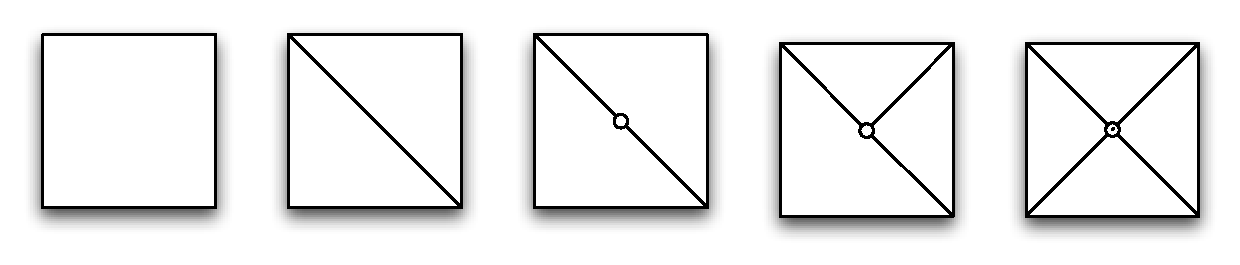
\includegraphics[scale=0.18]{../../../graphdod/quadtype.pdf}
   \end{center}
  \caption{}
\label{fig:quadtype}
\end{floatingfigure}



\FIXX{Is this definition of tame Voronoi hypermaps
compatible with what is stated in \cite{arx}? It looks quite different.
Can we make property $8$ of \cite[p.46]{arx} part of the linear programming specification
rather than the graph generator?  Choices are more easily accommodated then.}

\subsection{classification}\label{sec:class}

There is an archive of tame Voronoi hypermaps \cite{code}.  This
archive contains fewer than $2000$ hypermaps.\FIXX{Is this an accurate bound?}  

Two hypermaps $(D,e,n,f)$ and $(D',e',n',f')$ are properly isomorphic if there
is a bijection between $D$ and $D'$ that is equivariant for the face, node, and
edge permutations.  Each hypermap $(D,e,n,f)$ has a mirror image:
  $$
  (D,f n, n^{-1},f^{-1}).
  $$
  An improper
isomorphism between two hypermaps is a proper isomorphism between one hypermap and the
mirror image of the other.
Two hypermaps are isomorphic if there is a proper or improper isomorphism between
the two hypermaps. If a hypermap is involutive or planar, then so is every isomorphic
hypermap.

\begin{theorem}  If $H$ is a tame Voronoi hypermap, then it is isomorphic to
some hypermap in the archive.
\end{theorem}

The proof of this theorem relies on the piece of 
computer code described in Section~\ref{sec:gg}.  The reader is referred to that section
for a description of the details of the theorem.

\subsection{counterexamples are tame Voronoi hypermaps}

The following theorem proves that every potential counterexample to the Dodecahedral
conjecture gives a tame Voronoi hypermap.  In particular, the classification
in this section gives an explicit case enumeration of the possible combinatorial structures
of a counterexample.  The following section will eliminate each case in the enumeration.
This will eliminate all possible counterexamples to the Dodecahedral conjecture.

\begin{theorem}  Assume that $\Lambda$ is a counterexample to the Dodecahedral
conjecture.  (Without loss of generality,  assume that $0\in\Lambda=\Lambda(0,2t_{dod})$;
that the cardinality of $\Lambda^*$ is at least $13$; that $G(\Lambda)$ is biconnected.)  Let $H=(D,e,n,f)$ be the hypermap attached to the graph $G(\Lambda)$.
 For every dart $x\in D$ in face $F$, set
$$w(x) = \mu(\Lambda,U_F).$$
Then $H$ is a tame Voronoi hypermap and $w$ is a Voronoi weight assignment on $H$.
\end{theorem}



Since the definition of tame Voronoi hypermap is a long enumeration of different properties,
the proof of this theorem breaks into a long enumeration of lemmas, each establishing
one property.  The statement of the theorem specifies the weight assignment $w$.  The
verification that $w$ is a Voronoi weight, breaks into separate lemmas for each property in the definition.  The article \cite{arx} devotes
many pages to the proofs of these lemmas.  This articles sketches the proofs and
refers the reader to the fuller version for details.
Turn to an item by item discussion of the properties.  The first several
are elementary.

\subsubsection{involutive}
{\it The hypermap $H$ is involutive and planar.}  This has been established in Section~\ref{sec:ph}.


\subsubsection{connected}
{\it The set of darts $D$  is a single orbit under $\tangle{e,n,f}$.}  This is also
contained in Section~\ref{sec:ph}. It follows directly from the
connectedness of $G(\Lambda)$.

\subsubsection{simple}

{\it Every face of $H$ meets every node of $H$ in at most
dart.}  This is a direct consequence of the biconnectedness of $G(\Lambda)$.
Indeed, if by following the face permutation $x,f x, f^2 x,\ldots, f^r x= y$,
the darts $x\ne y$ lie at the same node $v$; then $v$ is an articulation vertex
of $G(\Lambda)$, and the graph is not biconnected.

\subsubsection{13}

{\it The number of nodes is at least $13$.}  This is a consequence of the assumption
that the cardinality of $\Lambda^*$ is at least $13$ and the bijection in
Section~\ref{sec:ph} between nodes of the hypermap and $\Lambda^*$.

\subsubsection{face cardinality}\label{sec:face}

{\it The cardinality of each face of $H$ is at least $3$ and at most $7$.}


By  definition, the face map on a dart $x$ takes the form
\begin{equation}\label{eqn:fx}
x = (0,v,w,u),\quad
f x = (0,w,\sigma_w^{-1}v,v),\quad
f^{-1} x = (0,u,v,\sigma_u v).
\end{equation}
In a biconnected graph with more than two vertices,
every vertex has degree at least two.
Thus every node of the hypermap has degree
at least two.  Thus, $\sigma_u v\ne v$ and $f x\ne f^{-1} x$.
Also, $w,u\in E(v)$, which does not contain $v$.  Thus, 
the form of $x,fx$, and 
$f^{-1} x$
in (\ref{eqn:fx}) shows these darts are distinct, and
the
face contains at least three distinct darts.

If some face of $H$ has cardinality at least $8$, then by Theorem~\ref{thm:main}
$$
\mu(\Lambda) =\sum_{U\in [Y(\Lambda)]}\mu(\Lambda,U) > t_8 =\mu(\Lambda_{dod}).
$$
Thus, $\Lambda$ is not a counterexample, as was assumed.

\subsubsection{degree}

{\it The degree of a node of type $(p,q,r)$ is at most five if $r>0$.}

\FIXX{I do not see a mention of this in \cite{arx}, but I have the impression
that it is needed for the graph generator.}

\subsubsection{degrees}\label{sec:degrees}

{\it The degree of each node of $H$ is at least $2$ and at most $6$.}


Section~\ref{sec:face} has already shown that the degrees are at least $2$.

Let $(p,q,r)$ be the type of node $v$.  If $r>0$, then the previous
property bounds the degree at five.  Assume $r=0$.  The
proof in this case is deferred until Section~\ref{sec:pq}.

\subsubsection{triangle types}

{\it Let $v_1,v_2,v_3$ be any three nodes of $H$ such that $v_i$ is adjacent to $v_j$
for each $i\ne j$.  Then there is a dart $x_i\in v_i$ such that $\{x_1,x_2,x_3\}$ is
a face of $H$.}

This is a restatement of Lemma~\ref{lemma:enclosed} in terms of the combinatorial
properties of hypermaps.


\subsubsection{adjacent degrees}

{\it There are never two nodes of type $(4,0,0)$ that are adjacent to one another.}

If there are two adjacent nodes of type $(4,0,0)$, then the graph takes the
shape of Figure~\ref{fig:adj4}.  This is an impossible configuration in a packing $\Lambda$
for purely geometric reasons.  It has nothing to do with the value of $\mu(\Lambda)$
and volumes of truncated Voronoi cells.
The impossibility proof appears as \cite[Lemma~3.8]{arx}. It is a reparametrization
of \cite[Prop.4.2]{Part1}.  This is one of the most delicate reparametrizations.

% XX Draw figure.  This is a simple figure showing two adjacent 4,0,0 type vertices.
\begin{floatingfigure}{30mm}
  \begin{center}
  %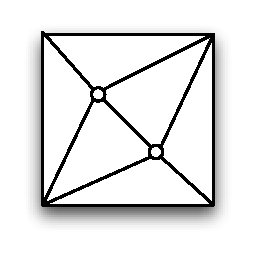
\includegraphics[scale=0.18]{../../../graphdod/adj4.pdf}
   \end{center}
  \caption{}
\label{fig:adj4}
\end{floatingfigure}


\subsubsection{quadrilateral types}


{\it Let $v_1,v_2,v_3,v_4$ be any four nodes of $H$ such that $v_i$ is adjacent
to $v_{i+1}$ for $i=1,2,3,4$ (setting $v_5=v_1$).  Then darts $x_i\in v_i$ can be chosen
so that the faces containing $x_i$ fall into one of the four patterns depicted
in Figure~\ref{fig:quadtype}.}

Let $G'$ be the spherical graph on the vertex set $\{v_1,v_2,v_3,v_4\}$
whose edge set forms a cycle $\{v_i,v_{i+1}\}$ for $i=1,2,3,4$.  Then by
Jordan curve theorem for polygons, $Y(G')$ consists of two connected components.
The result of \cite[Lemma~3.8]{arx} cited in the previous proof states more precisely
that exactly one connected component $U$ of $Y(G')$ has solid angle less than $2\pi$,
and that $U\cap\Lambda$ contains at most one point.

If $U\cap\Lambda$ is empty, then the first pattern of Figure~\ref{fig:quadtype} occurs.

Assume that $U\cap\Lambda$ contains a single point $v_0\in\Lambda$.  Again, by
the Jordan curve theorem and the planarity of $G(\Lambda)$, 
all edges $\{v_0,u\}$ in $G(\Lambda)$ have the form
$\{v_0,v_i\}$ for $i=1,2,3,4$.  Every node is known to have degree
at least $2$.  Thus,  $v_0$ is adjacent to $2$, $3$, or $4$ of the vertices $v_i$.
Figure~\ref{fig:quadtype} gives all such connection patterns of $v_0$ with $v_i$, except
the one shown in Figure~\ref{fig:tripent}.  

%\begin{figure}[htb]
%  \centering
%  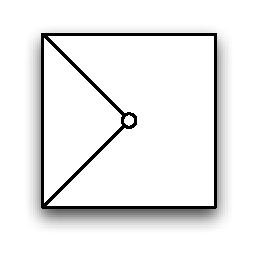
\includegraphics[scale=0.80]{../../../graphdod/tripent.pdf}
%  \caption{a pattern to be excluded}
%\label{fig:tripent}
%\end{figure}

\begin{floatingfigure}{25mm}
  \begin{center}
  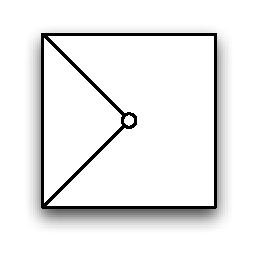
\includegraphics[scale=0.80]{../../../graphdod/tripent.pdf}
  \end{center}
  \caption{}
\label{fig:tripent}
\end{floatingfigure}




Thus, it is enough to show that pattern of Figure~\ref{fig:tripent} does not occur 
in any counterexample to the Dodecahedral conjecture.  This graph contains a triangle
$F$ and a pentagon $F'$, with corresponding connected components
$U=U_F$ and $U'=U_{F'}\in[Y(\Lambda)]$.
An important estimate \cite[Lemma~10.1]{arx} gives that
$$
\mu(\Lambda,U) + \mu(\Lambda,U') > 0.168.
$$
If there is some other face  with $n\ge 4$ sides, then 
Theorem~\ref{thm:main} gives
$$
\mu(\Lambda) \ge \mu(\Lambda,U)+\mu(\Lambda,U') + t_n \ge 0.168 + 0.031 > \mu(\Lambda_{dod}).
$$
Otherwise, pick any four vertices in $\Lambda^*$ other than $v_0,v_1,\ldots,v_4$.  Let $U_1,\ldots,U_r$ be the connected components
indexed by triangles of $G(\Lambda)$
that contain one of these four vertices.  
Another estimate \cite[Lemma~5.2]{arx} gives
$$
\sum_{i=1}^r \mu(\Lambda,U_i) \ge 4 (0.004) \text{ and hence }
\mu(\Lambda) \ge 0.168 + 4(0.004) > \mu(\Lambda_{dod}).
$$
This shows that $\Lambda$ is not a counterexample.


\subsubsection{weight assignment}

{\it There exists a Voronoi weight assignment of total weight at most $\mu(\Lambda_{dod})$.}

By definition, a counterexample $\Lambda$ is a packing such that
\begin{equation}\label{eqn:178}
\mu(\Lambda)=\sum_{U\in [Y(\Lambda)]} \mu(\Lambda,U) \le \mu(\Lambda_{dod}).
\end{equation}
The set of connected components $[Y(\Lambda)]$ is in bijection with the faces of $H$.
By the definition of $w$ in the statement of the theorem, (\ref{eqn:178}) can
be rewritten as
$$
\sum_{x\in[D/f]} w(x) \le \mu(\Lambda_{dod}).
$$
This is exactly what it means for $w$ to have total weight at most $\mu(\Lambda_{dod})$.

\subsubsection{Voronoi weight}\label{sec:pq}

{\it The weight assignment $w$ is a Voronoi weight.}

This can be expressed as the following claims.
\begin{enumerate}
\item If the face $F$  has cardinality $n\ge3$ then $\mu(\Lambda,U_F)\ge t_n$.
\item Let $F\subset D$ 
be any face with cardinality $m \ge 4$.  Let $y\in F$.
Let $V$ be a set of vertices of $F$, such
that no two are adjacent to one another.  
Assume that the type of each node of $V$ is $(4,0,1)$.
Let $X$ be the set of triangles at the vertices $V$.
that is, the set of darts in nodes in $V$ except those in $F$.
Let $m'$ be the cardinality of $V$.
Then
\begin{equation}\label{eqn:m'}
\mu(\Lambda,U_F) + \sum_{F'\in X} \mu(\Lambda,U_{F'}) \ge t_m  +  0.016 m'.
\end{equation}
\item If the node of $x$ has type $(p,q,0)$ and degree $m=p+q$, then
  \begin{equation}\label{eqn:pq}
  \sum_{i=1}^m \mu(\Lambda,U_i) \ge b(p,q).
  \end{equation}
\end{enumerate}

The first of these claims is a direct consequence of Theorem~\ref{thm:main}.
Consider the second claim.  Form the graph $G'(\Lambda)$ and
partition $U_F$ into subcomponents 
by the algorithm described in Section~\ref{sec:sub}.  A result
in Tarski arithmetic states that two internal pairs $\{u,w\}$
and $\{u',w'\}$ with $|u-w|,|u'-w'|\le\sqrt8$ do not cross
each other in the sense of Section~\ref{sec:sub}.  (See \cite[exact ref~XX]{arx}.)  It follows that every internal pair $\{u,w\}$ such that
$|u-w|\le\sqrt8$ forms an edge of the graph $G'$.
The bound on $t_m$ is obtained by supperadditivity, from a collection
of inequalities $\mu(\Lambda,U_i)>D_{dod}(n,k)$ for each subcomponent.

Let $v$  be a node in $V$.  Let $(0,v,u,w)$ be the dart in $F$
at node $v$.  Let $U_v$ be the subcomponent indexed by the
triangle $\{v,u,w\}$ in $G'$.
At a node of type $(4,0,1)$, the pair $\{u,w\}$ is necessarily internal.
Let $U'_1,\ldots,U'_4$ be the standard components indexed
by the four triangles at $v$. 
By summing over $V$, the following two inequalities
imply (\ref{eqn:m'}).
\begin{enumerate}
\item If $|u-w|>\sqrt8$, then
   $$
   \sum_{i=1}^4\mu(\Lambda,U'_i) > 0.016.
   $$
\item If $|u-w|\le\sqrt8$, then
   $$
   \mu(\Lambda,U_v)+ \sum_{i=1}^4\mu(\Lambda,U'_i) > D_{dod}(3,1) + 0.016.
   $$
\end{enumerate}
These inequalities are obtained by summing over interval arithmetic
inequalities for each term $\mu(\Lambda,\cdot)$.   
A detailed proof appears at \cite[Theorem~8.1]{arx}.


Consider the final claim.  
The argument at \cite[p.14]{arx} goes as follows.
Let $v\in\Lambda^*$ be a vertex.
Type is $(p,q,0)$ means that there are $p$ triangles and $q$ quadrilaterals
in the graph $G(\Lambda)$ at the vertex $v$.
Interval arithmetic can be used to compute lower and upper bounds on the
azimuth angles $\op{azim}(U_F,v)$ when $U_F$ is a triangle or quadrilateral.
These bounds are \cite[F.2.1,F.4]{arx}
$$
\begin{array}{lrlll}
\text{triangle:} &  0.856147 &< \op{azim}(U,v) &< 1.88673,\\
\text{quadrilateral:} & 1.15242 &< \op{azim}(U,v) &< 3.25887.\\
\end{array}
$$
\begin{equation}\label{eqn:2pi}
\sum^m \op{azim}(U_i,v) = 2\pi.
\end{equation}
By the bounds on the azimuth angles, this equality can only be satisfied for
special $(p,q)$. Anything else is a geometric impossibility.  The feasible pairs $(p,q)$
are listed in \cite[Lemma~6.1]{arx}.  According to this list, $p\le 7$ and $q\le 5$.

Interval arithmetic methods establish a list of nonlinear inequalities relating
$\op{azim}(U_F,v)$ to $\mu(\Lambda,U_F)$ when $F$ is a triangle or quadrilateral \cite[exact ref~XX]{code}.
If free variables $\optt{azim}(F)$ and $\optt{mu(F)}$ are substituted into these inequalities
for  $\op{azim}(U_F,v)$ and $\mu(\Lambda,U_F)$, then the resulting inequalities are
linear in these variables.   A system of linear inequalities results. 
(This is the method of linear relaxation.)  A lower bound
on the left-hand side of (\ref{eqn:pq}) is the solution of the linear program
$$
\min \sum_F \optt{mu(F)}
$$
subject to 
$$
\sum_F \optt{azim(F)} = 2\pi,
$$
and to the system of linear inequalities.  The linear program is run for
each $p,q$ and a constant $b(p,q)$ slightly smaller than the minimization was picked.
This gives the table of values.

If $\Lambda$ is a counterexample to the Dodecahedral conjecture with a vertex
of type $(p,q,0)$, then
$$\mu(\Lambda_{dod}) \ge \mu(\Lambda) > b(p,q).$$
An inspection of the list of constants $b(p,q)$ in the table shows that that this implies
that $p+q\le 6$.  That is, the degree of every vertex of type $(p,q,0)$
is at most $6$.  This
is the property needed in Section~\ref{sec:degrees}.



\section{Linear Programs}

This section discusses Theorem~\ref{thm:graph-system}.  It is one of
the main steps in the proof of the Dodecahedral conjecture.
The discussion begins with the terminology used in the
statement of the theorem.


\begin{definition} A hypermap system is a pair $(H,\Phi)$,
where $H=(D,e,n,f)$ is a hypermap, and $\Phi$ is a finite set constraints on $H$.  More precisely, let $V$ be the vector space of
real-valued functions on $D$.  A finite set of constraints $\Phi$ is a finite
set of boolean valued functions $\phi:V^\ell\to \{\op{true},\op{false}\}$
for some $\ell$. (Assume $\ell$ is independent of $\phi\in \Phi$).
\end{definition}

The hypermap system $(H,\Phi)$ is said to be feasible, if
there is some $x=(x_1,\ldots,x_\ell)\in V^\ell$ such that
$\phi(x)$ holds for all $\phi\in\Phi$. Otherwise,  
the system is infeasible.

Appendix~\ref{ap:A} gives a finite set of constraints $\Phi_{dod}$, 
specified
in a uniform way for every tame Voronoi hypermap $H$.  
We call this particular hypermap system
the {\it Voronoi hypermap system}. 
This determines,
for every tame Voronoi hypermap $H$, a well-defined extension
to a hypermap system $(H,\Phi_{dod})$.   


\begin{theorem}\label{thm:graph-system}  Let 
$H$ be any tame Voronoi hypermap. 
Then $(H,\Phi_{dod})$ is infeasible.
\end{theorem}

This proof is carried out by computer as a collection of linear
programs.  This is one of the three major parts of the proof
of the Dodecahedral conjecture that has been carried out by computer.
This article describes the relationship between the
feasibility of $(H,\Phi)$ and a linear programming feasibility
problem.  It also describes some details of the implementation of 
the code.

Section~\ref{sec:class} enumerates of all tame Voronoi
hypermap systems.  Thus, the proof of
Theorem~\ref{thm:graph-system} may proceed case by case.


Let's focus attention for a moment on one tame Voronoi hypermap $H=(D,e,n,f)$ and the corresponding Voronoi hypermap system $(H,\Phi)$.
A simple strategy will show that it is infeasible.
For some $\ell\in\ring{N}$,
each constraint $\phi$ is a function on $V^\ell$, where $V$ is
the vector space of real-valued functions on $D$.  Thus,
$V^\ell$ can be identified with $\ring{R}^m$, where $m= \ell \#(D)$.
An inspection of the form of the constraints $\phi\in \Phi$, as listed
in Appendix~\ref{ap:A}, reveals they all have a 
very special form.  They are all linear constraints
on $\ring{R}^m$.  

Some of the linear constraints
carry guard conditions.  That is, some constraints have the form
  \begin{equation}\label{eqn:guard}
  (A x < b)  \Rightarrow (A' x \le b'),
  \end{equation}
for $x\in\ring{R}^m$, and various matrices $A,A'$ and vectors
$b,b'$.  (The vector inequality $a \le b$ means
that $a_i\le b_i$ for every component of the vectors $a,b$.)
The constraint $(A x < b)$ is called a guard condition.
Variations are allowed in which some of the inequalities in the
guard condition are weak and some of the inequalities in the
consequent are strict.

The collection of all inequalities that do not have a guard 
condition is a system of linear inequalities.  Standard linear
programming packages can be used to determine whether this
system of linear inequalities has a feasible solution.  If this
linear program is infeasible, then the hypermap system $(H,\Phi)$
is clearly also infeasible.  When this happens, a
proof of the infeasibility of $(H,\Phi)$ results.

When this fails, the constraints with guard conditions are
used.
The introduction of a constraint that has a nontrivial guard condition
involves multiple steps.  
The constraint (\ref{eqn:guard}) can be rewritten in logically
equivalent form as
  $$
   (A_{1} x \ge b_{1}) \lor \cdots \lor
   (A_{r} x \ge b_{r}) \lor (A' x \le b'),
  $$
where $A_{i}$ and $b_{i}$ are the rows of $A$ and $b$.
Taking each disjunct in turn, one linear inequality at a time
is added to the system
of linear inequalities, and the resulting system is shown to be
infeasible.  When each
systems are infeasible, then $(H,\Phi)$ itself is infeasible.

In general, more than one guarded constraint may be added.  If
$k$ constraints are added with $r_1,\ldots,r_k$ guards
respectively, then as many as $(r_1+1)\cdots (r_k+1)$ systems
of linear equalities are created.  If they are all infeasible,
then $(H,\Phi)$ itself is infeasible.\FIXX{Perhaps there is
never more than one guard constraint in use at a time.  If so,
delete this paragraph.}

This discussion may give the impression 
that a great many linear programming feasibility
problems are created in this manner.  In practice, nearly all
of the hypermap systems are eliminated in the first pass, without
requiring recourse to the guarded conditions.  



\subsection{counterexample implies feasibility}

\begin{theorem}\label{thm:feasible}  Let $\Lambda$ be a counterexample to the Dodecahedral conjecture.  Let $(H,\Phi)$ be the Voronoi hypermap system attached to $\Lambda$.
Then $(H,\Phi)$ is feasible.
\end{theorem}

\begin{proof}  It is enough to give some assignment of the variables
$\optt{sol},\ldots$ that satisfies the predicates $\Phi$, defined
in Appendix~\ref{ap:A}.  The notation has been set up in a way that
suggests the assignment.  
Let $\alpha = (0,v,u,w)$ be a dart.  Let $F$ be the face containing $\alpha$. Make the following settings.
$$
\begin{array}{llllllllllll}
\optt{yn}(\alpha) & \optt{ye}(\alpha) & \optt{sol}(\alpha) & \optt{azim}(\alpha) & \optt{mu}(\alpha) & \optt{omega}(\alpha) \\
|v|               & |v-u|           & \sol(U_F)   & \op{azim}(U_F,v) & \mu(\Lambda,U_F) & \omega(\Lambda,U_F).\\
\end{array}
$$

All of the predicates $\Phi$ can be shown to hold for this assignment,
either as a consequence of definitions, as consequences of geometrical facts, or
as consequences of interval arithmetic calculations.
The first group of predicates hold by definition and convention.
%
% XX This needs to be typed into the Appendix, using Obua's format.
The predicates in Section~\ref{sec:multi} hold by \cite[Lemma~5.2]{arx}.
%
All inequalities from Sections~\ref{sec:tri} to the end of the
Appendix hold by interval arithmetic.

The interval arithmetic calculations for the predicates with guard
conditions were verified in two stages.  
The polygonal face is triangulated, and
the standard component $U_F$ is partitioned in a corresponding
way into parts $U_1,\ldots,U_k$.
In the first stage,
the guard hypotheses were used to obtain interval
arithmetic bounds on the lengths of the internal edges of the triangulation.
In the second stage, these edge length bounds are used as hypotheses
in further interval arithmetic bounds that give lower bounds on
$\omega(\Lambda,U_i) > c_i$.  Then
  $$\omega(\Lambda,U_F) = \sum_{i=1}^k\omega(\Lambda,U_i) >\sum_{i=1}^k c_i.$$
This becomes a general predicate on darts of the form:
$$
\optt{omega}(\alpha) > c.
$$
\end{proof}


\section{Appendix: Voronoi Hypermap System}\label{ap:A}

This appendix  lists the system of constraints determining
the Voronoi hypermap system.  As the main body of the text explains
a hypermap system is a pair $(H,\Phi)$, where $H$ is a hypermap
and $\Phi$ is a finite set of constraints on $H$.  To describe
the constraints $\Phi$ in precise terms requires some notation.

Let $H=(D,e,n,f)$ be a hypermap.   Greek letters
$\alpha,\beta \in D$ denote darts.  Let $V$ be the vector space 
of real-valued  functions on $D$.  A constraint $\phi$ is a boolean-valued function on $V^\ell$ for some $\ell$.  The suggestive
notation $(\optt{sol},\optt{mu},\optt{tau},\optt{yn},\optt{ye})\in V^\ell$  is used for $\ell$-tuples
of elements of $V$.  The main text relates each coordinate back
with its namesake.  For example, the linear constraints on
$\optt{sol}\in V$, mirror  nonlinear relations satisfied by the
nonlinear function $\sol$ in the main text.  This correspondence
between functions in $V$ and functions does not enter into the
definition of the Voronoi hypermap system.  For the purposes of this
appendix, this correspondence is simply an aid to the
intuition.

If $m$ is  a permutation on $D$, let $\op{ord}(m,\alpha,i)$
be the predicate that asserts that the cardinality of the $m$-orbit
of $\alpha$ is $i\in\ring{N}$.
\bigskip


\subsection{general bounds and relations}\label{sec:lpbounds}


\subsubsection{variable bounds}

$$
\begin{array}{lll}
\leftalign\\
   \forall \alpha\in D.\\
    2 \le \optt{yn}(\alpha) \sland
    \optt{yn}(\alpha) \le 2t_{dod} \\
    2 \le \optt{ye}(\alpha) \sland
    \optt{ye}(\alpha) \le 2t_{dod}\\
   0 \le \optt{sol}(\alpha) \sland
     \optt{sol}(\alpha) \le 4 \pi \\
   0 \le \optt{azim}(\alpha) \sland
     \optt{azim}(\alpha) \le 2\pi \\
   0 \le \optt{mu}(\alpha) \sland
% upper bound 0.2, comes from 0.178 < 0.2.
      \optt{mu}(\alpha) \le 0.2 \\
   0 \le \optt{omega}(\alpha) \sland
      \optt{omega}(\alpha) \le 6.0 \\   
% omega = mu+0.42755 sol < 0.2+ 0.42755 4pi < 6 
\end{array}
$$

\subsubsection{definitional}
$$
\begin{array}{lll}
\leftalign\\
   \forall \alpha\in D.\\
  \optt{yn}(\alpha) = \optt{yn}(n\alpha) \\
  \optt{ye}(\alpha) = \optt{ye}(e\alpha) \\
  \optt{omega}(\alpha) = \optt{omega}(f\alpha) \\
  \optt{mu}(\alpha) = \optt{mu}(f\alpha) \\
  \optt{sol}(\alpha)= \optt{sol}(f\alpha) \\
  \optt{mu}(\alpha) = \optt{omega}(\alpha) - 0.42755\ \optt{sol}(\alpha) \\
\end{array}
$$

\subsubsection{geometric relations}

The angles around each vertex sum to $2\pi$.  Girard's formula
for the area of a spherical polygon holds.
$$
\begin{array}{lll}
\leftalign\\
\forall \alpha\in D.\\ 
   \optt{ord}(n,\alpha,k) \Rightarrow
   \sum_{i=1}^k \optt{azim}(n^i\alpha )  = 2\pi.\\
   \optt{ord}(f,\alpha,k) \Rightarrow
   \sum_{i=1}^k \optt{azim}(f^i\alpha ) = \optt{sol} + (k -2)\pi.\\
   \end{array}
$$

\subsubsection{counterexample property}

\noindent
Let $D'\subset D$ be a set of representatives of the faces in $D$.
A counterexample to the Dodecahedral conjecture satisfies
$\omega(\Lambda) \le \omega(\Lambda_{dod})$.  This becomes part
of the Voronoi hypermap system as the linear inequality:
$$
\begin{array}{lll}
\leftalign\\
\sum_{\alpha\in D'} \optt{omega}(\alpha) \le 5.5503 \\
\end{array}
$$
\FIXX{Check the constant 5.5503 against what the LPs use.
It should be strictly larger than $\omega(\Lambda_{dod})$.}

\subsubsection{the main estimate}
$$
\begin{array}{lll}
\leftalign\\
\forall \alpha\in D.\\
   \optt{ord}(f,\alpha,4) \Rightarrow
   \optt{mu}(\alpha) > 0.031 \\
   \optt{ord}(f,\alpha,5) \Rightarrow
   \optt{mu}(\alpha) > 0.076 \\
   \optt{ord}(f,\alpha,6) \Rightarrow
   \optt{mu}(\alpha) > 0.121 \\
   \optt{ord}(f,\alpha,7) \Rightarrow
   \optt{mu}(\alpha) > 0.166 \\
\end{array}
$$




\subsection{triangle interval arithmetic constraints}\label{sec:tri}

Interval arithmetic gives the following bounds.
$$
\begin{array}{lll}
\leftalign\\
  \forall \alpha\in D. \ \op{ord}(f,\alpha,3) 
   \Rightarrow \\ 
      \optt{omega}(\alpha) > 0.202804  \sland \\
   \optt{sol}(\alpha) > 0.315696 \sland \\
   \sol(S) < 1.051232\\
   \optt{azim}(\alpha) > 0.856147\\
   \optt{azim}(\alpha) < 1.886730\\
   \optt{mu}(\alpha) > 0
\end{array}
$$

$$
\begin{array}{lll}
\leftalign\\
\forall\alpha\in D. \ \op{ord}(f,\alpha,3) \Rightarrow \\
   \optt{omega}(\alpha) - 0.68\ \optt{sol}(\alpha) + 1.88718\ \optt{azim}(\alpha) > 1.54551 \\
   \optt{omega}(\alpha) - 0.68\ \optt{sol}(\alpha) + 0.90746\ \optt{azim}(\alpha) > 0.706725\\
   \optt{omega}(\alpha) - 0.68\ \optt{sol}(\alpha) + 0.46654\ \optt{azim}(\alpha) > 0.329233\\
   \optt{omega}(\alpha) - 0.55889\ \optt{sol}(\alpha) - 0\ \optt{azim}(\alpha) > -0.0736486\\
   \optt{omega}(\alpha) - 0.63214\ \optt{sol}(\alpha) - 0\ \optt{azim}(\alpha) > -0.13034\\
   \optt{omega}(\alpha) - 0.73256\ \optt{sol}(\alpha) - 0\ \optt{azim}(\alpha) > -0.23591\\
   \optt{omega}(\alpha) - 0.89346\ \optt{sol}(\alpha) - 0\ \optt{azim}(\alpha) > -0.40505\\
   \optt{omega}(\alpha) - 0.3\ \optt{sol}(\alpha) - 0.5734\ \optt{azim}(\alpha) > -0.978221\\
   \optt{omega}(\alpha) - 0.3\ \optt{sol}(\alpha) - 0.03668\ \optt{azim}(\alpha) > 0.024767\\
   \optt{omega}(\alpha) - 0.3\ \optt{sol}(\alpha) + 0.04165\ \optt{azim}(\alpha) > 0.121199\\
   \optt{omega}(\alpha) - 0.3\ \optt{sol}(\alpha) + 0.1234\ \optt{azim}(\alpha) > 0.209279\\
   \optt{omega}(\alpha) - 0.42755\ \optt{sol}(\alpha) - 0.11509\ \optt{azim}(\alpha) > -0.171859\\
   \optt{omega}(\alpha) - 0.42755\ \optt{sol}(\alpha) - 0.04078\ \optt{azim}(\alpha) > -0.050713\\
   \optt{omega}(\alpha) - 0.42755\ \optt{sol}(\alpha) + 0.11031\ \optt{azim}(\alpha) > 0.135633\\
   \optt{omega}(\alpha) - 0.42755\ \optt{sol}(\alpha) + 0.13091\ \optt{azim}(\alpha) > 0.157363\\
   \optt{omega}(\alpha) - 0.55792\ \optt{sol}(\alpha) - 0.21394\ \optt{azim}(\alpha) > -0.417998\\
   \optt{omega}(\alpha) - 0.55792\ \optt{sol}(\alpha) - 0.0068\ \optt{azim}(\alpha) > -0.081902\\
   \optt{omega}(\alpha) - 0.55792\ \optt{sol}(\alpha) + 0.0184\ \optt{azim}(\alpha) > -0.051224\\
   \optt{omega}(\alpha) - 0.55792\ \optt{sol}(\alpha) + 0.24335\ \optt{azim}(\alpha) > 0.193993\\
   \optt{omega}(\alpha) - 0.68\ \optt{sol}(\alpha) - 0.30651\ \optt{azim}(\alpha) > -0.648496\\
   \optt{omega}(\alpha) - 0.68\ \optt{sol}(\alpha) - 0.06965\ \optt{azim}(\alpha) > -0.278\\
   \optt{omega}(\alpha) - 0.68\ \optt{sol}(\alpha) + 0.0172\ \optt{azim}(\alpha) > -0.15662\\
   \optt{omega}(\alpha) - 0.68\ \optt{sol}(\alpha) + 0.41812\ \optt{azim}(\alpha) > 0.287778\\
   \optt{omega}(\alpha) - 0.64934\ \optt{sol}(\alpha) - 0\ \optt{azim}(\alpha) > -0.14843\\
   \optt{omega}(\alpha) - 0.6196\ \optt{sol}(\alpha) - 0\ \optt{azim}(\alpha) > -0.118\\
   \optt{omega}(\alpha) - 0.58402\ \optt{sol}(\alpha) - 0\ \optt{azim}(\alpha) > -0.090290\\
   \optt{omega}(\alpha) - 0.25181\ \optt{sol}(\alpha) - 0\ \optt{azim}(\alpha) > 0.096509\\
   \optt{omega}(\alpha) - 0.00909\ \optt{sol}(\alpha) - 0\ \optt{azim}(\alpha) > 0.199559\\
   \optt{omega}(\alpha) + 0.93877\ \optt{sol}(\alpha) - 0\ \optt{azim}(\alpha) > 0.537892\\
   \optt{omega}(\alpha) + 0.93877\ \optt{sol}(\alpha) - 0.20211\ \optt{azim}(\alpha) > 0.27313\\
   \optt{omega}(\alpha) + 0.93877\ \optt{sol}(\alpha) + 0.63517\ \optt{azim}(\alpha) > 1.20578\\
   \optt{omega}(\alpha) + 1.93877\ \optt{sol}(\alpha) - 0\ \optt{azim}(\alpha) > 0.854804\\
   \optt{omega}(\alpha) + 1.93877\ \optt{sol}(\alpha) - 0.20211\ \optt{azim}(\alpha) > 0.621886\\
   \optt{omega}(\alpha) + 1.93877\ \optt{sol}(\alpha) + 0.63517\ \optt{azim}(\alpha) > 1.57648\\
   \optt{omega}(\alpha) - 0.42775\ \optt{sol}(\alpha) - 0\ \optt{azim}(\alpha) > -0.000111\\
   \optt{omega}(\alpha) - 0.55792\ \optt{sol}(\alpha) - 0\ \optt{azim}(\alpha) > -0.073037\\
   \optt{omega}(\alpha) - 0\ \optt{sol}(\alpha) - 0.07853\ \optt{azim}(\alpha) > 0.08865\\
   \optt{omega}(\alpha) - 0\ \optt{sol}(\alpha) - 0.00339\ \optt{azim}(\alpha) > 0.198693\\
   \optt{omega}(\alpha) - 0\ \optt{sol}(\alpha) + 0.18199\ \optt{azim}(\alpha) > 0.396670\\
   \optt{omega}(\alpha) - 0.42755\ \optt{sol}(\alpha) - 0.2\ \optt{azim}(\alpha) > -0.332061\\
   \optt{omega}(\alpha) - 0.3\ \optt{sol}(\alpha) - 0.36373\ \optt{azim}(\alpha) > -0.58263\\
   \optt{omega}(\alpha) - 0.3\ \optt{sol}(\alpha) + 0.20583\ \optt{azim}(\alpha) > 0.279851\\
   \optt{omega}(\alpha) - 0.3\ \optt{sol}(\alpha) + 0.40035\ \optt{azim}(\alpha) > 0.446389\\
   \optt{omega}(\alpha) - 0.3\ \optt{sol}(\alpha) + 0.83259\ \optt{azim}(\alpha) > 0.816450\\
   \optt{omega}(\alpha) - 0.42755\ \optt{sol}(\alpha) - 0.51838\ \optt{azim}(\alpha) > -0.932759\\
   \optt{omega}(\alpha) - 0.42755\ \optt{sol}(\alpha) + 0.29344\ \optt{azim}(\alpha) > 0.296513\\
   \optt{omega}(\alpha) - 0.42755\ \optt{sol}(\alpha) + 0.57056\ \optt{azim}(\alpha) > 0.533768\\
   \optt{omega}(\alpha) - 0.42755\ \optt{sol}(\alpha) + 1.18656\ \optt{azim}(\alpha) > 1.06115\\
   \optt{omega}(\alpha) - 0.55792\ \optt{sol}(\alpha) - 0.67644\ \optt{azim}(\alpha) > -1.29062\\
   \optt{omega}(\alpha) - 0.55792\ \optt{sol}(\alpha) + 0.38278\ \optt{azim}(\alpha) > 0.313365\\
   \optt{omega}(\alpha) - 0.55792\ \optt{sol}(\alpha) + 0.74454\ \optt{azim}(\alpha) > 0.623085\\
   \optt{omega}(\alpha) - 0.55792\ \optt{sol}(\alpha) + 1.54837\ \optt{azim}(\alpha) > 1.31128\\
   \optt{omega}(\alpha) - 0.68\ \optt{sol}(\alpha) - 0.82445\ \optt{azim}(\alpha) > -1.62571\\
\end{array}
$$

Introduce abbreviations $y_1 = \optt{yn}(\alpha)$, $y_2 = \optt{yn}(f \alpha)$,
$y_3 = \optt{yn}(f^2 \alpha)$, $y_4 = \optt{ye}(\alpha)$, $y_5 = \optt{ye}(f\alpha)$, $y_6 = \optt{ye}(f^2\alpha)$.

$$
\begin{array}{lll}
\leftalign\\
\forall\alpha\in D. \ \op{ord}(f,\alpha,3) \Rightarrow \\
  \optt{sol}(\alpha) > 0.551285 - 0.245 (y_1+y_2+y_3-6) + 0.063 (y_4+y_5+y_6-6)\\
  \optt{sol}(\alpha) > 0.551285 - 0.3798 (y_1+y_2+y_3-6) + 0.198 (y_4+y_5+y_6-6)\\
  \optt{sol}(\alpha) < 0.551286 - 0.151 (y_1+y_2+y_3-6) + 0.323 (y_4+y_5+y_6-6)\\

  \optt{mu}(\alpha) > 0.0392 (y_1+y_2+y_3-6) + 0.0101 (y_4+y_5+y_6-6) \\
  \optt{omega}(\alpha) > 0.235702 -0.107 (y_1+y_2+y_3-6) + 0.116 (y_4+y_5+y_6-6)\\
  \optt{omega}(\alpha) > 0.235702 -0.0623 (y_1+y_2+y_3-6) + 0.0722 (y_4+y_5+y_6-6)\\
  \optt{azim}(\alpha) > 1.23095 + 0.237 (y_1-2) - 0.372 (y_2+y_3+y_5+y_6-8) + 0.708 (y_4-2) \\
  \optt{azim}(\alpha) > 1.23095 + 0.237 (y_1-2) - 0.363 (y_2+y_3+y_5+y_6-8) + 0.688 (y_4-2)\\
  \optt{azim}(\alpha) < 1.23096 + 0.505 (y_1-2) - 0.152(y_2+y_3+y_5+y_6-8) + 0.766 (y_4-2)\\

\end{array}
$$

\subsection{quadrilateral interval arithmetic bounds}\label{sec:quad}

Interval arithmetic gives the following bounds.
$$
\begin{array}{lll}
\leftalign\\
\forall\alpha\in D. \ \op{ord}(f,\alpha,4) \Rightarrow \\
   \optt{omega}(\alpha) > 0.455149\\
   \optt{sol}(\alpha) > 0.731937\\
   \optt{sol}(\alpha) < 2.85860\\
   \optt{azim}(\alpha) > 1.15242\\
   \optt{azim}(\alpha) < 3.25887\\
   \optt{mu}(\alpha) > 0.031350\\
\end{array}
$$


$$
\begin{array}{lll}
\leftalign\\
\forall\alpha\in D. \ \op{ord}(f,\alpha,4) \Rightarrow \\
   \optt{omega}(\alpha) - 0.42775\ \optt{sol}(\alpha) - 0.15098\ \optt{azim}(\alpha) > -0.3670\\
   \optt{omega}(\alpha) - 0.42775\ \optt{sol}(\alpha) - 0.09098\ \optt{azim}(\alpha) > -0.1737\\
   \optt{omega}(\alpha) - 0.42775\ \optt{sol}(\alpha) - 0.00000\ \optt{azim}(\alpha) > 0.0310\\
   \optt{omega}(\alpha) - 0.42775\ \optt{sol}(\alpha) + 0.18519\ \optt{azim}(\alpha) > 0.3183\\
   \optt{omega}(\alpha) - 0.42775\ \optt{sol}(\alpha) + 0.20622\ \optt{azim}(\alpha) > 0.3438\\
   \optt{omega}(\alpha) - 0.55792\ \optt{sol}(\alpha) - 0.30124\ \optt{azim}(\alpha) > -1.0173\\
   \optt{omega}(\alpha) - 0.55792\ \optt{sol}(\alpha) - 0.02921\ \optt{azim}(\alpha) > -0.2101\\
   \optt{omega}(\alpha) - 0.55792\ \optt{sol}(\alpha) - 0.00000\ \optt{azim}(\alpha) > -0.1393\\
   \optt{omega}(\alpha) - 0.55792\ \optt{sol}(\alpha) + 0.05947\ \optt{azim}(\alpha) > -0.0470\\
   \optt{omega}(\alpha) - 0.55792\ \optt{sol}(\alpha) + 0.39938\ \optt{azim}(\alpha) > 0.4305\\
   \optt{omega}(\alpha) - 0.55792\ \optt{sol}(\alpha) + 2.50210\ \optt{azim}(\alpha) > 2.8976\\
   \optt{omega}(\alpha) - 0.68000\ \optt{sol}(\alpha) - 0.44194\ \optt{azim}(\alpha) > -1.6264\\
   \optt{omega}(\alpha) - 0.68000\ \optt{sol}(\alpha) - 0.10957\ \optt{azim}(\alpha) > -0.6753\\
   \optt{omega}(\alpha) - 0.68000\ \optt{sol}(\alpha) - 0.00000\ \optt{azim}(\alpha) > -0.4029\\
   \optt{omega}(\alpha) - 0.68000\ \optt{sol}(\alpha) + 0.86096\ \optt{azim}(\alpha) > 0.8262\\
   \optt{omega}(\alpha) - 0.68000\ \optt{sol}(\alpha) + 2.44439\ \optt{azim}(\alpha) > 2.7002\\
   \optt{omega}(\alpha) - 0.30000\ \optt{sol}(\alpha) - 0.12596\ \optt{azim}(\alpha) > -0.1279\\
   \optt{omega}(\alpha) - 0.30000\ \optt{sol}(\alpha) - 0.02576\ \optt{azim}(\alpha) > 0.1320\\
   \optt{omega}(\alpha) - 0.30000\ \optt{sol}(\alpha) + 0.00000\ \optt{azim}(\alpha) > 0.1945\\
   \optt{omega}(\alpha) - 0.30000\ \optt{sol}(\alpha) + 0.03700\ \optt{azim}(\alpha) > 0.2480\\
   \optt{omega}(\alpha) - 0.30000\ \optt{sol}(\alpha) + 0.22476\ \optt{azim}(\alpha) > 0.5111\\
   \optt{omega}(\alpha) - 0.30000\ \optt{sol}(\alpha) + 2.31852\ \optt{azim}(\alpha) > 2.9625\\
   \optt{omega}(\alpha) - 0.23227\ \optt{azim}(\alpha) > -0.1042\\
   \optt{omega}(\alpha) + 0.07448\ \optt{azim}(\alpha) > 0.5591\\
   \optt{omega}(\alpha) + 0.22019\ \optt{azim}(\alpha) > 0.7627\\
   \optt{omega}(\alpha) + 0.80927\ \optt{azim}(\alpha) > 1.5048\\
   \optt{omega}(\alpha) + 5.84380\ \optt{azim}(\alpha) > 7.3468\\
\end{array}
$$

\subsection{multiface conditions}\label{sec:multi}

\FIXX{Add the inequalities in the format of Obua page 71,
the multiface inequalities, see page 14 McL 2003, Lemma 5.2,
Theorem 8.1 vertex adjustments.  
}


\subsection{guard conditions}\label{sec:guard}

\FIXX{This section is not finished.  There follows a sample of the format
envisioned for the inequalities with guards, (page 65).  The proofs
are explained in an earlier section.  It is not necessary to list
all the bounds obtained on diagonals.  They are not part of the LP specs.}

\noindent
Condition H.14.1:  % Use alpha= y1.
$$
\begin{array}{lll}
\leftalign\\
\forall \alpha\in D.\\
  \op{ord}(f,\alpha,5) \sland 
  \optt{azim}(\alpha) < 1.342 \sland
  \optt{azim}(f^3\alpha) < 1.684 \sland
  \optt{yn}(\alpha) < 2.153 \sland \\
   \optt{y}(f\alpha) < 2.174 \sland
  \optt{yn}(f^2\alpha) < 2.26 \sland
  \optt{yn}(f^3 \alpha) < 2.194 \sland
  \optt{yn}(f^4 \alpha) < 2.314  \\
  \Rightarrow
  \optt{omega}(\alpha) > 0.950
\end{array}
$$

\noindent
Condition H.14.2:  \FIXX{Potential problem, in H.14.1, the
condition is $y(10)< 2.26$, the index changes in H.14.2
to $y(5) > 2.26$.}
$$
\begin{array}{lll}
\leftalign\\
\forall \alpha\in D.\\
  \op{ord}(f,\alpha,5) \sland 
  \optt{azim}(\alpha) < 1.342 \sland
  \optt{azim}(f^3\alpha) < 1.684 \sland
  \optt{y}(\alpha) < 2.153 \sland \\
   \optt{y}(f\alpha) < 2.174 \sland
  \optt{y}(f^2\alpha) \ge 2.26 \sland
  \optt{y}(f^3 \alpha) < 2.194 \sland
  \optt{y}(f^4 \alpha) < 2.314  \\
   \Rightarrow
  \optt{mu}(\alpha) > 0.1234
\end{array}
$$
